\documentclass[a4paper,12pt]{article}

\usepackage[utf8]{inputenc}
\usepackage[T1]{fontenc}
\usepackage[czech]{babel}
\usepackage{amsmath}
\usepackage{amsfonts}
\usepackage{amssymb}
\usepackage{graphicx}
\usepackage{hyperref}
\usepackage{float}
\usepackage{hyperref}

\usepackage[a4paper]{geometry}
\geometry{verbose,tmargin=2.5cm,bmargin=2cm,lmargin=2cm,rmargin=2cm}
\usepackage{fancyhdr}
\pagestyle{fancy}

% nastaven� pisma a �e�tiny
\usepackage{lmodern}
\usepackage[T1]{fontenc}
% v�cesloupcov� tabulky
\usepackage{multirow}

% vno�en� popisky obr�zk�
\usepackage{subcaption}

% automatick� konverze EPS 
\usepackage{graphicx} 
\usepackage{epstopdf}

% odkazy a z�lo�ky


% Pozn�mky p�i p�ekladu
\usepackage{xkeyval}	% Inline todonotes
\usepackage[textsize = footnotesize]{todonotes}
\presetkeys{todonotes}{inline}{}


\title{Řešení úkolu pro TurtleBot s detekcí objektů a SLAM}
\author{Michal Bouda, Erik Doležal, Ondřej Váňa}
\date{\today}

\begin{document}

\maketitle

\tableofcontents

\section{Zadání}
Úkolem práce je napsat řešení úkolu, kde má Roomba TurtleBot kopnout míč do branky označené modrými pilíři.
Rozložení problému je vidět na obrázku \eqref{fig:map}.
\begin{figure}[H]
\centering
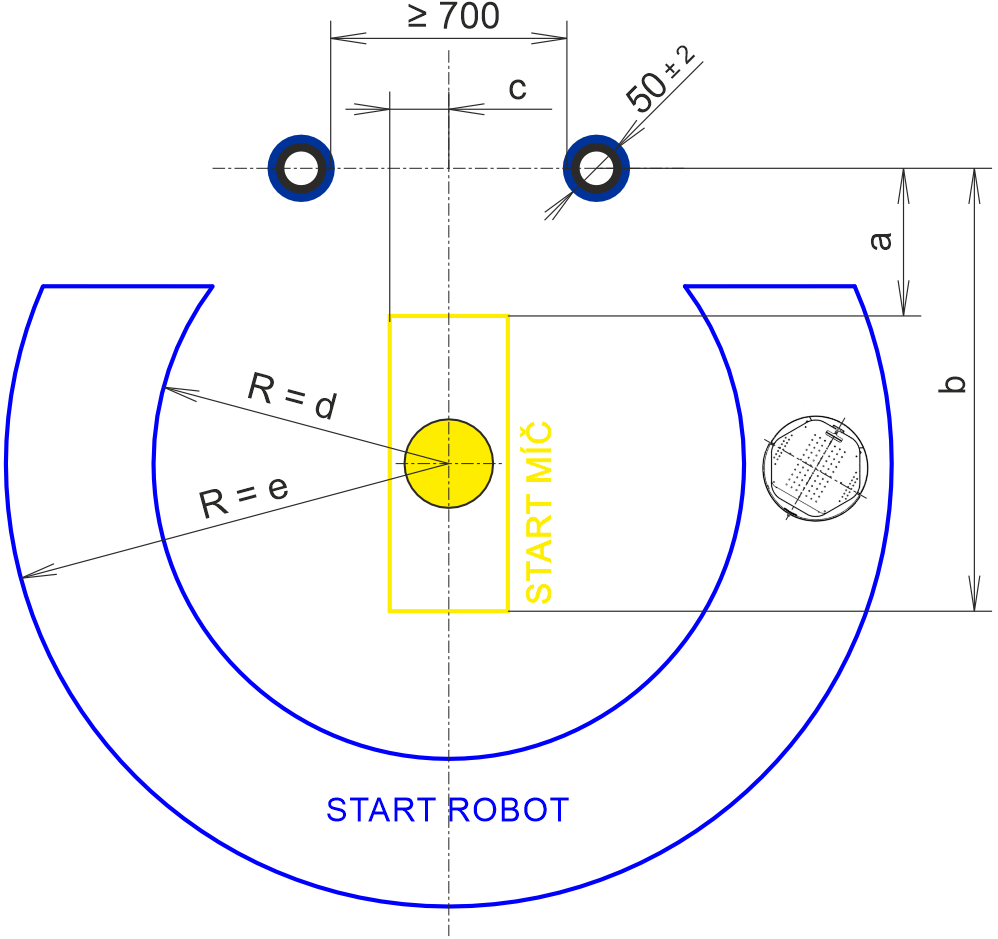
\includegraphics[width=0.4\textwidth]{pictures/map.png}
\caption{Rozložení objektů v prostoru (ze zedání)}
\label{fig:map}	
\end{figure}

\subsection{Úloha 2}
Robot má za úkol najít míč a ten kopnout mezi modré pilíře, které jsou od sebe vzdálené minimálně $700$ mm. Robot musí zastavit $20$ cm před brankou. Míč je vzdálen od osy branky maximálně $c = 150$ mm.
Míč se bude nacházet v minimální vzdálenosti $a = 500$ mm od brány a bude nejdále $b = 1,5$ m. TurtleBot bude na začátku umístěn od středu míče ve vzdálenosti $d = 0,7$ m až $e = 2,5$ m.
Za bránou může být neomezený počet pilířů.

\subsection{Úloha 3}
Od Úlohy 2 se Úloha 3 liší tím, že míč může být vzdálen od osy branky $c = 300$ mm. Vzdálenost míče od branky může být až $b = 2$ m.
Největším rozdílem je možnost výskutu až dvou překážek před čarou. Ty jsou umístěny tak, že pokaždé existuje cesta od míe k brance o minimální šířce $600$ mm.

\section{Řešení}
Naše řešení jsme rozdělili na tři hlavní části. První část je zpracování obrazu, druhá část je SLAM a třetí část je plánování a pohyb robota. Tyto části běží v hlavní smyčce programu. 
Po naimportování knihoven čeká robot na stisk tlačítka, které spustí hlavní smyčku. Splnění úkolu oznámí zvukovým signálem.

Naše řešení je dimenzováno pro řešení třetí úlohy. Z nedostataku času pro ošetření všech možných přídapů, jsme se ale rozhodli řešit druhou úlohu. 
Při řešení problému bylo využíváno nástroje GitHub Copilot pro jednoduché úkony pro zrychlení práce. 
\subsection{Zpracování obrazu}
Detekci objektů děláme pomocí konvoluční neuronové sítě YOLO \cite{YOLO} (You Only Look Once), kterou poté konvertujeme do ONNX \cite{ONNX}. Důvodem k použití CNN bylo, aby náše řešení dobře zvládalo změny v osvětlení a jiné rušivé vstupy jako například špinavý žlutý míč. Segementace obrazu pomocí barev, by mohla být v tomto ohledu nespolehlivá. Jako vstup používáme obraz z Intel RealSense D435 kamery.
\subsubsection{Trénování CNN}
YOLO model jsme museli nejdříve natrénovat na rozponávání pilířů a míče. Učinili jsme tak na více než 670 obrázcích,
které jsme pořídili pomocí kamery na robotovi. Dalších 120 jsme použili pro validaci. Obrázky jsme ručně anotovali pomocí programu Label Studio. Jak vypadá anotace je vidět v obrázku \eqref{fig:label_studio}.
\begin{figure}[H]
    \centering
    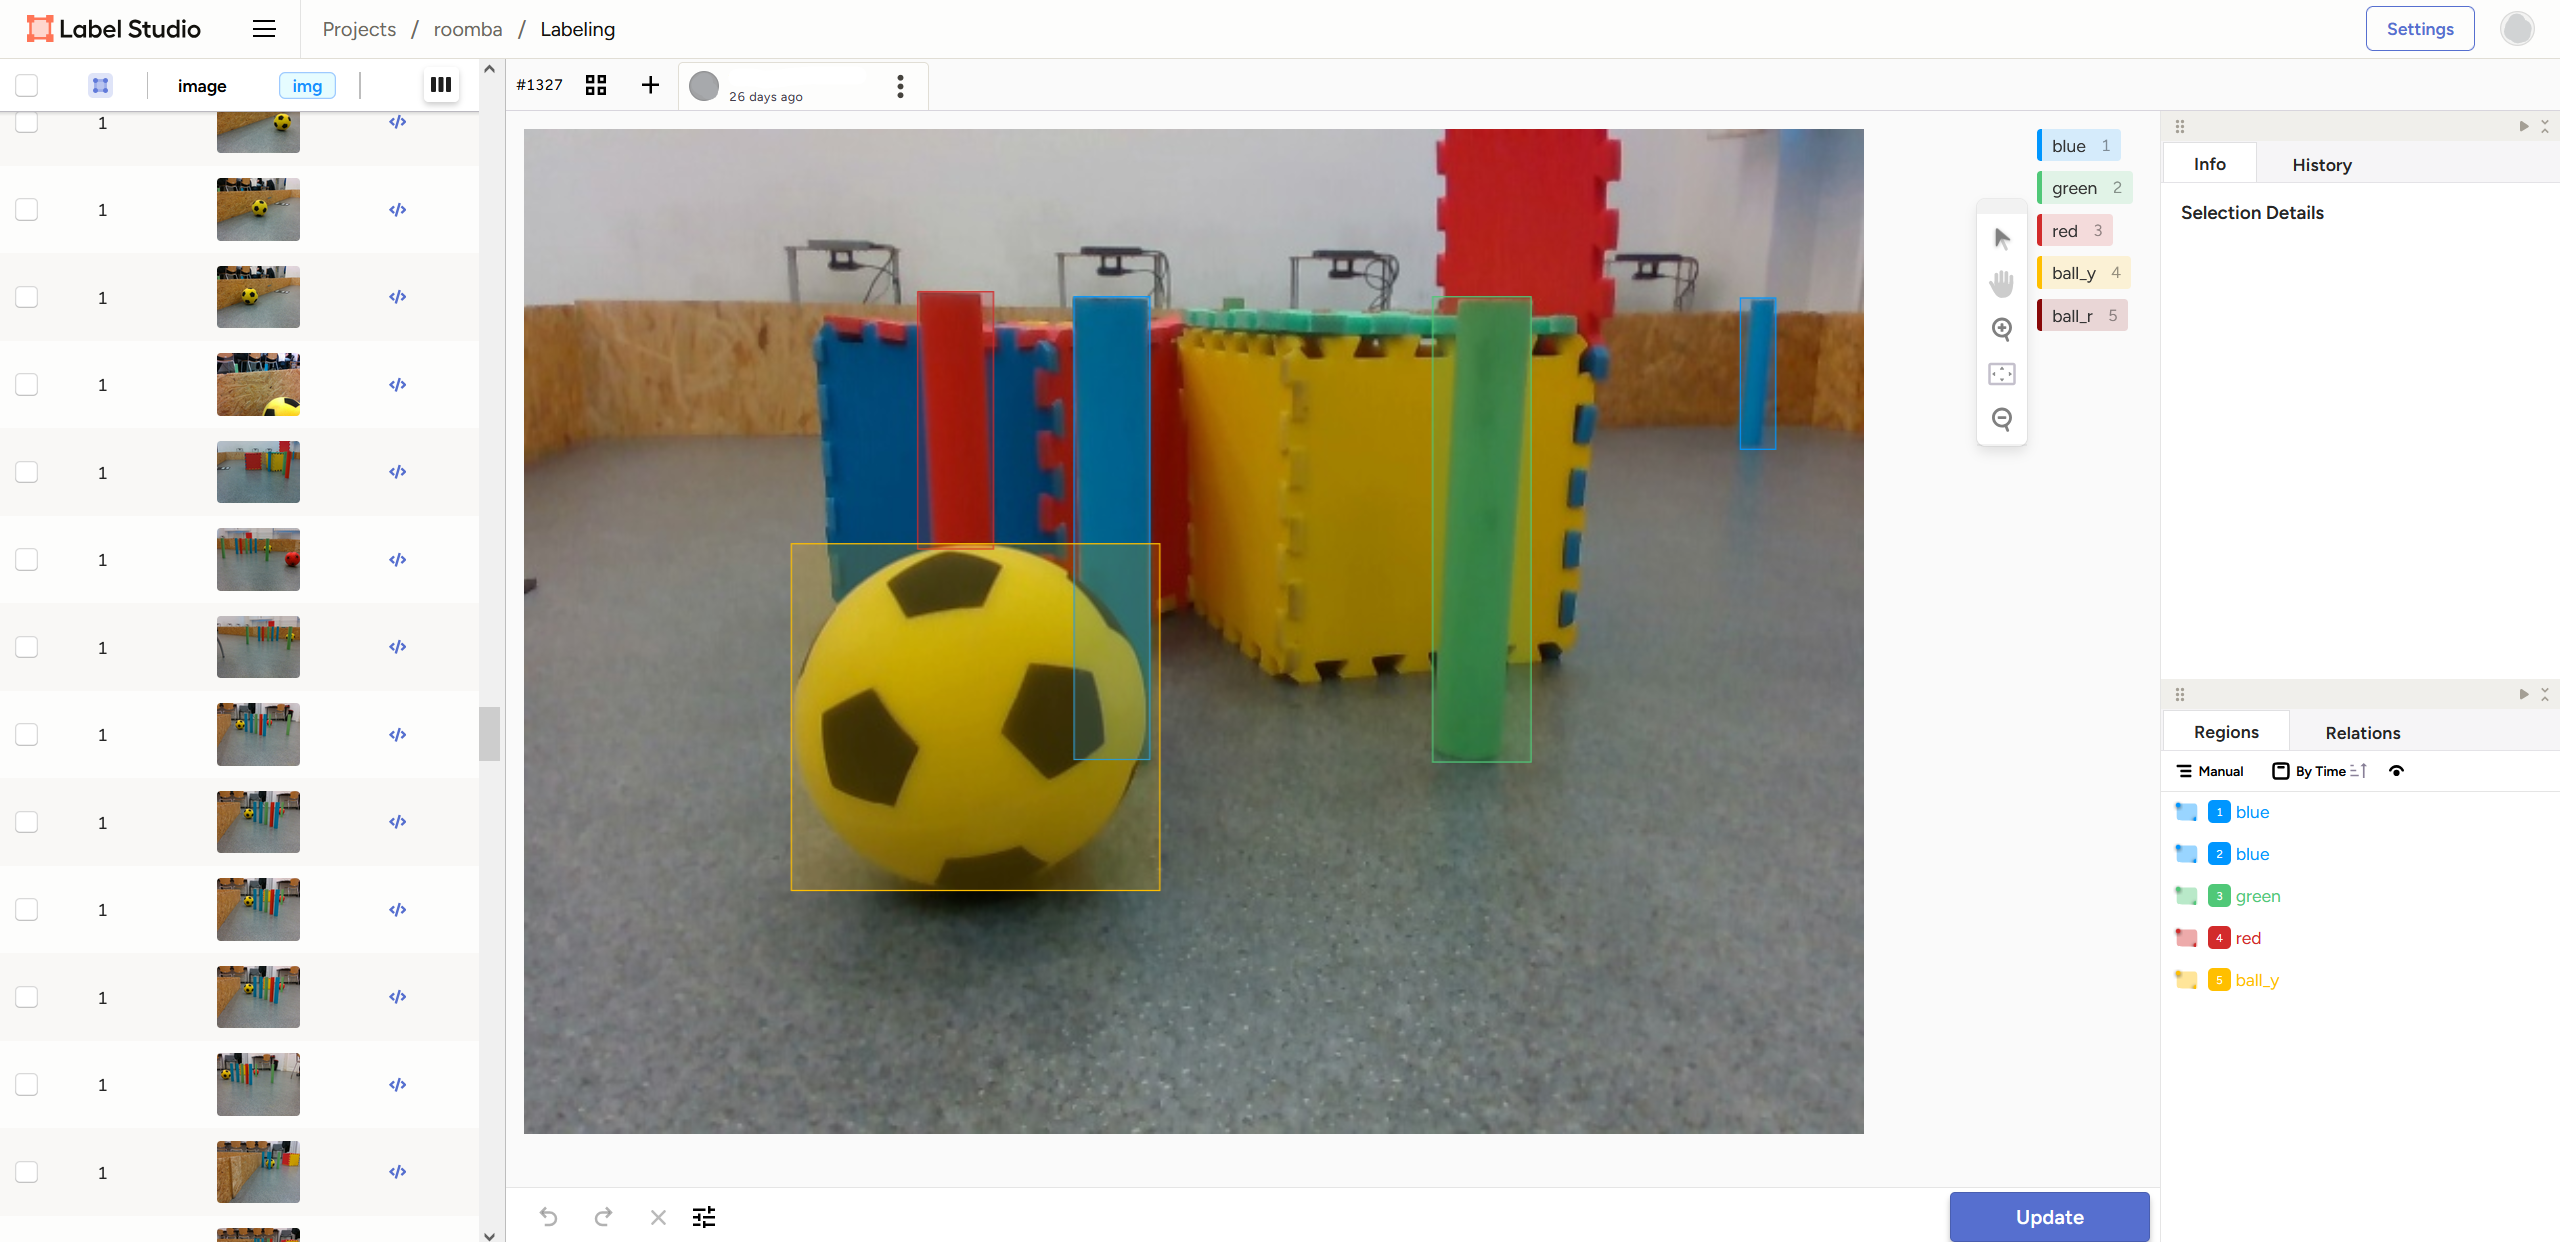
\includegraphics[width=0.8\textwidth]{pictures/label_studio.png}
    \caption{Anotování v Label Studiu}
    \label{fig:label_studio}	
\end{figure}
Pro anotaci jsme použili nastavení \textit{Object Detection with Bounding Boxes}, tedy jsme anotavali pomocí obdelníků. Zvolili jsme možnost bez rotace, všechny obdelníky mají tedy rovnoběžné strany se stranami obrazu. 
Možnost segmentace, myšleno maskou jsme zamítli z různých důvodou, např. pracné anotace. 
Anotovaný data set byl poté vyexportován ve formátu YOLO.
Pomocí Python kódu a knihovny od Ultralitics \cite{Ultralitics} jsme natrénovali model. Vyzkoušeli jsme YOLO verze v8 a 11. Ukázalo se, že verze 11 je mnohem přesnější, zvláště při změně osvětlení. 
Protože detekce musí probíhat rychle, zkoušeli jsme modeli 11s a 11n. I když je model 11s přesnější, používáme ho jen výjimečně, protože může způsobit problémy pro SLAM svojí dlouhou časovou náročností. I přesto máme natrénované dva modely v rozlišení 160p a 240p.
I pro model 11n jsme zkoušeli různé rozlišení. Rozlišení 160p a 240p bylo zpracováno dostatečně rychle a s uspokojivími výsledky. Oba modely byly natrénovany na 300 epochách.


\begin{figure}[H]
    \centering
    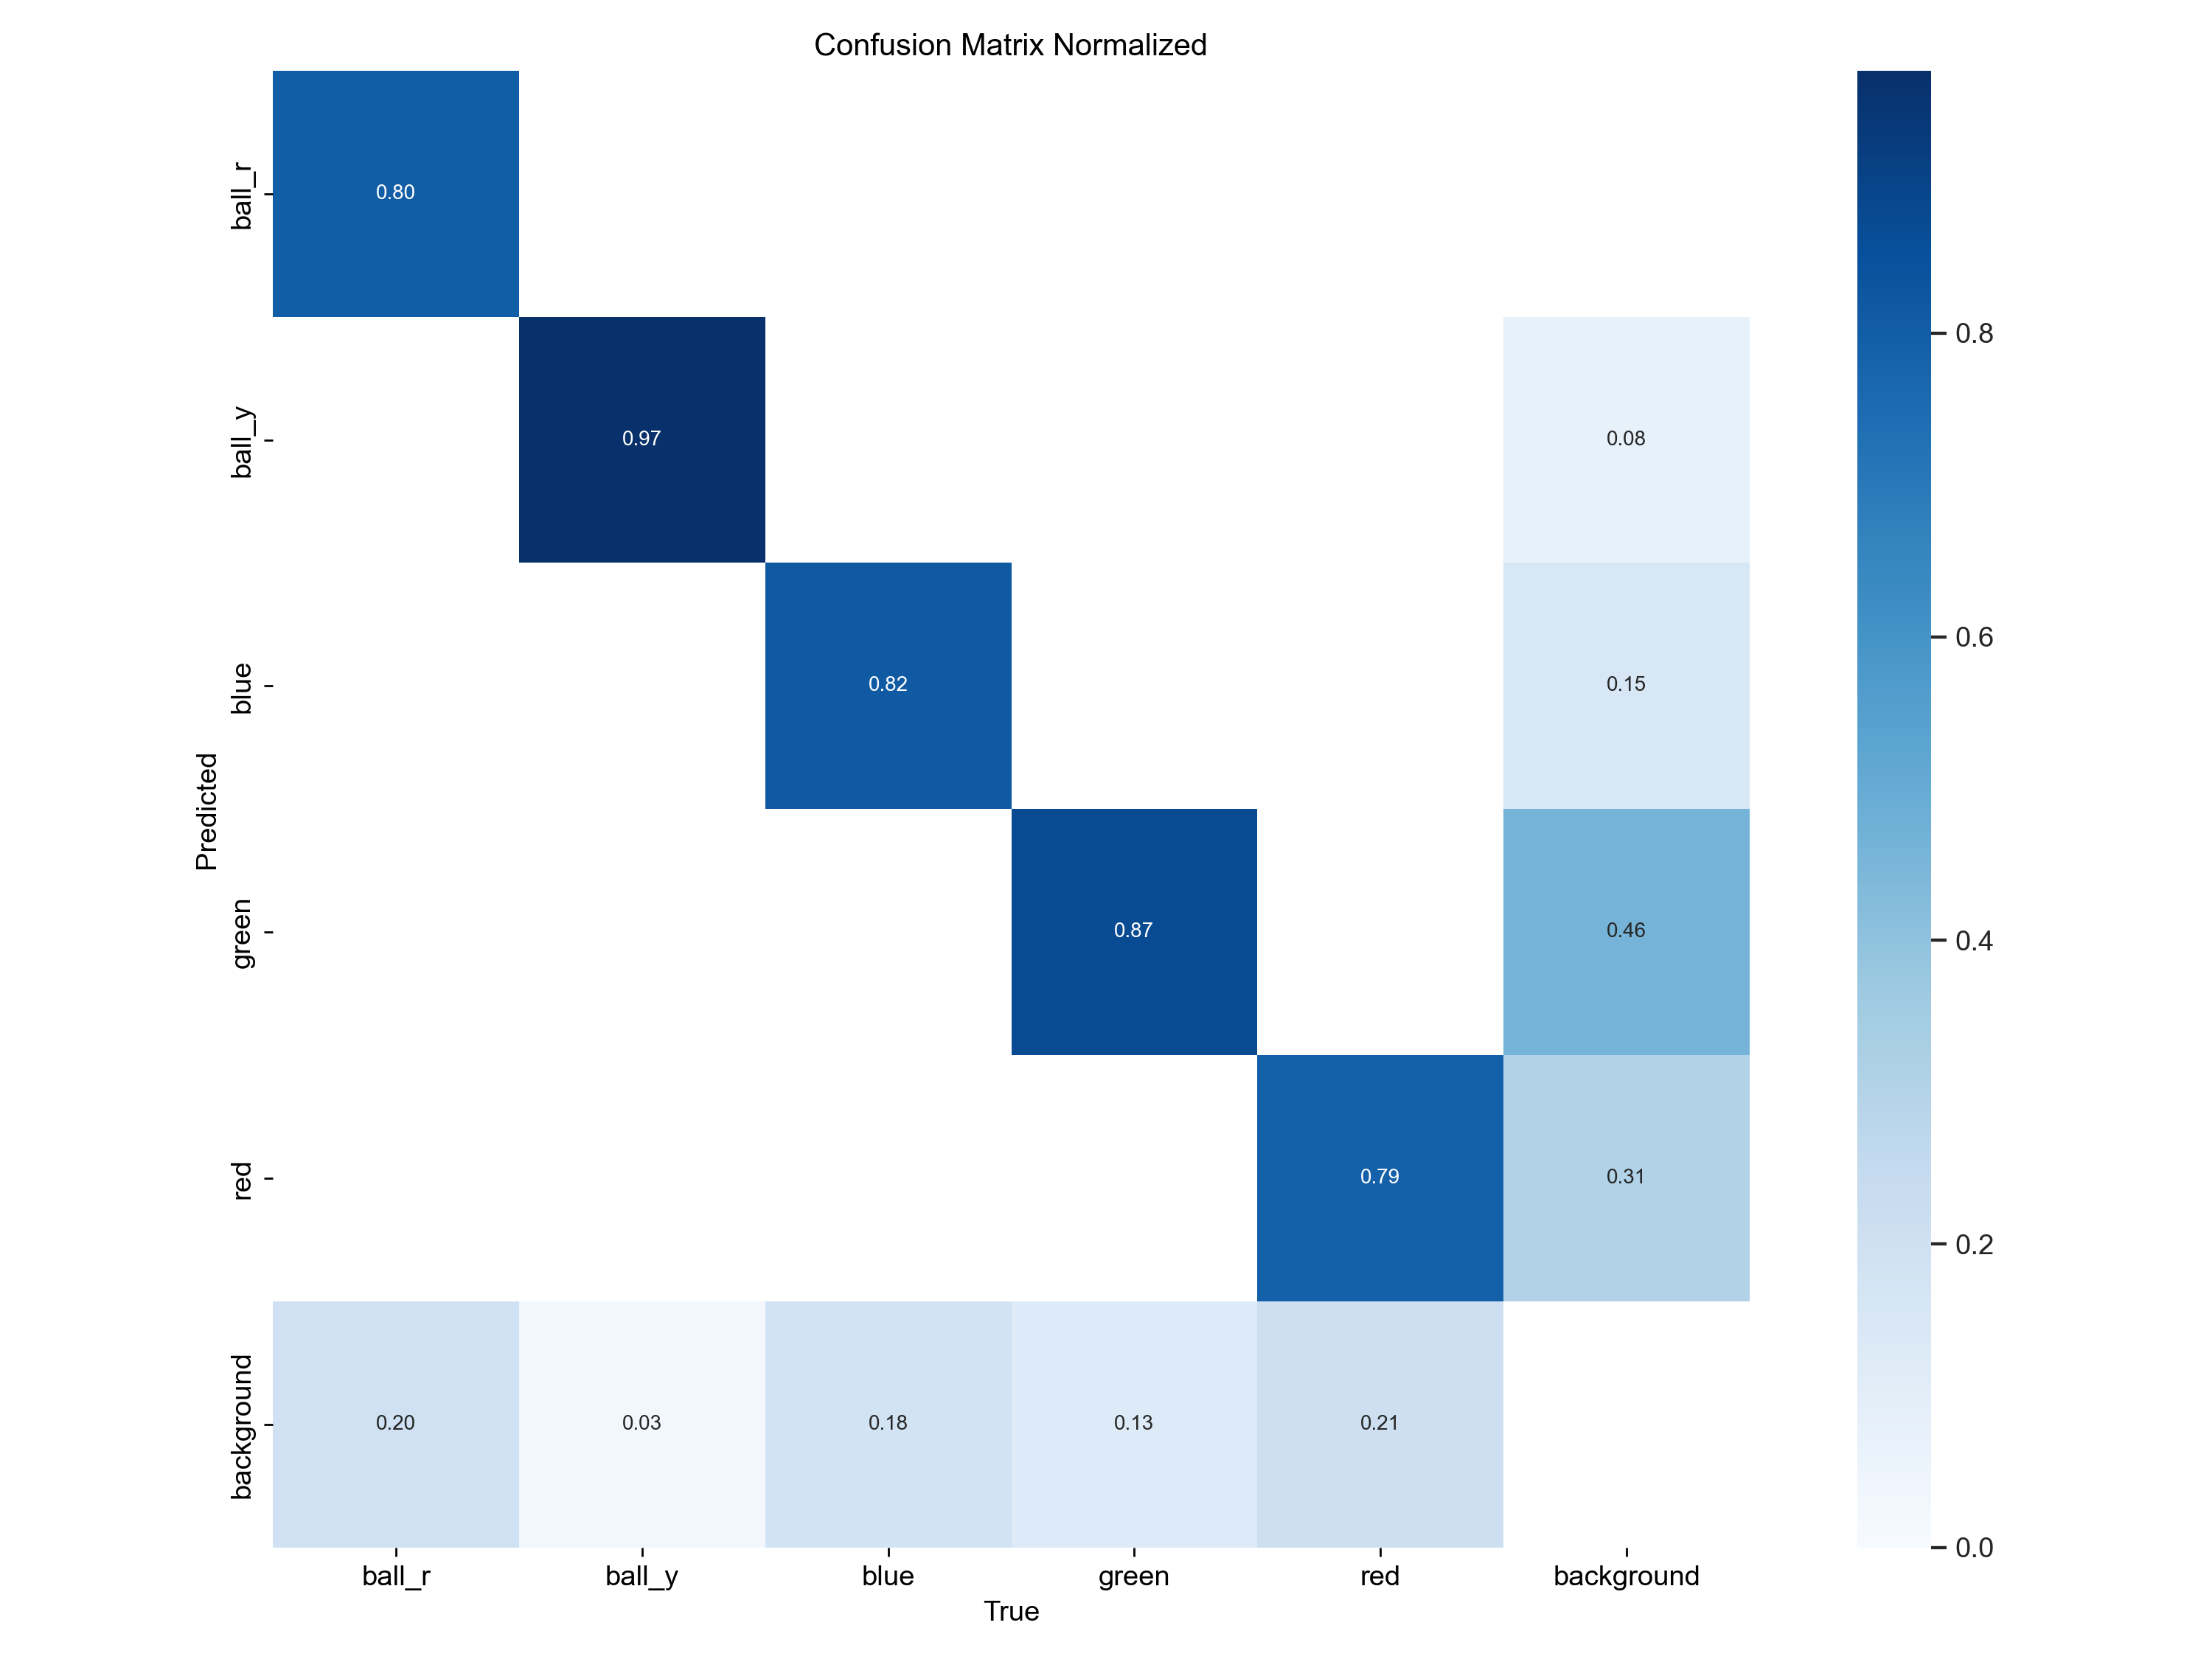
\includegraphics[width=0.8\textwidth]{pictures/v11n_160p.png}
    \caption{Normalizovaná matice záměn pro model 11n 160p}
    \label{fig:confusion_matrix_160p}
\end{figure}

\begin{figure}[H]
    \centering
    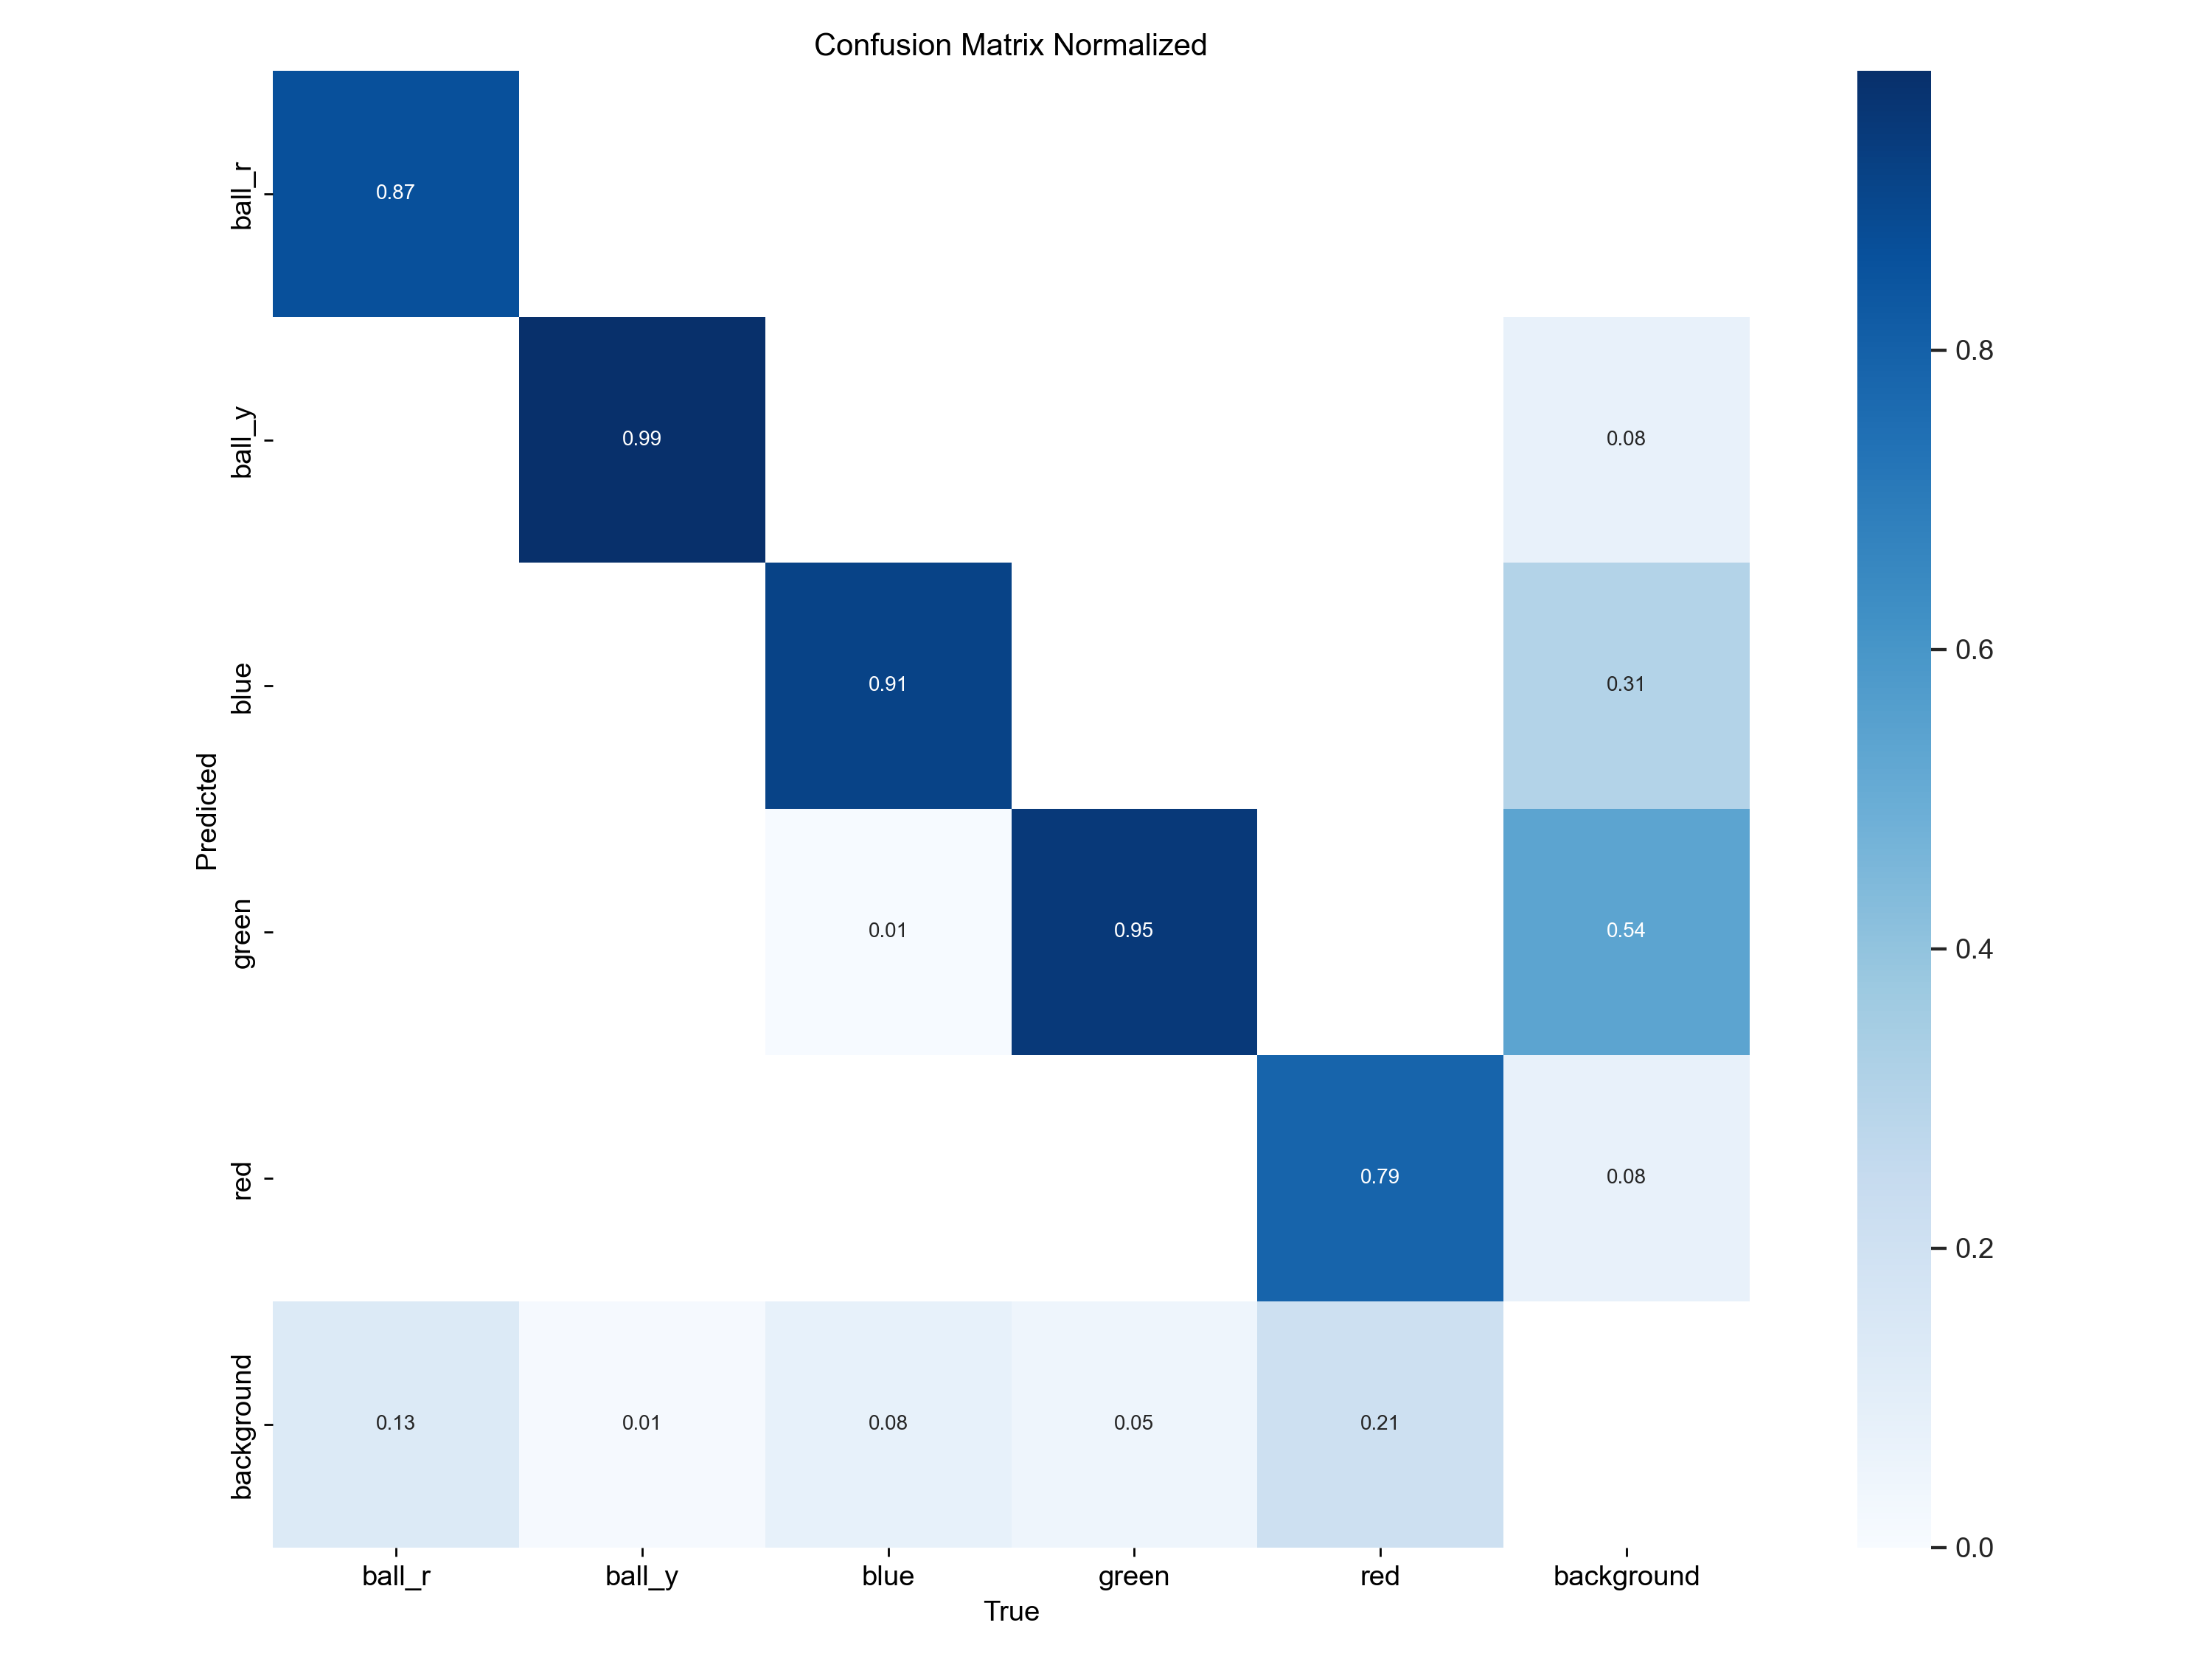
\includegraphics[width=0.8\textwidth]{pictures/v11n_240p.png}
    \caption{Normalizovaná matice záměn pro model 11n 240p}
    \label{fig:confusion_matrix_240p}
\end{figure}

Model 160p (Obrázek \eqref{fig:confusion_matrix_160p}) je v některých podmínkách znatelně horší oproti 240p (Obrázek \eqref{fig:confusion_matrix_240p}) v rozpoznávání modrých pilířů.
To může způsobit velké problémy, protože modré pilíře tvoří branku. Nejčastějším objektem, který byl zaměněn s pozadím, je zelený pilíř, který, když je detekován navíc, minimálně překaží úspěšnému vyřešení problému.

\subsubsection{Rozpoznávání obrazu}
K rozpoznávání použiváme buď model YOLO 11n při rozlišení 160p nebo při 240p v závislosti na prostředí a pokud více benefitujeme z rychlejší detekce nebo její přesnosti.
Na robotovi zajišťuje rozpoznávání class \texttt{Camera}. Třída má metodu \texttt{get detections}, která získá obraz z kamery. 
Seznam objektů vracíme pro potřeby SLAM jako numpy array poloha x, poloha y, objekt. Poloha x, y je poloha relativně k robotovi v prostoru.

K detekci nepoužíváme samotnou knihovnu YOLO. Model nejdříve konvertujeme do ONXX (Open Neural Network Exchange). Důvodem pro toto rozhodnutí je dlouhá doba, kdy YOLO knihovna zpracovála obraz. ONNX to zvládá rychleji z části díky tomu, že je optimalizovaná pro spouštění na procesoru.
Používání ONNX ale přineslo spoustu výzev, protože YOLO knihovna řešila spoustu věci za nás. Museli jsme naimplementovat počítaní pravděpodobností detekce pomocí softmax. 
Poté pomocí Non-Maximum Suppression z knihovny TorchVision řešíme odstranění duplicitních detekcí. A samozřejmostí je nepracování s detekcemi, které nedosahují nějaké hranice jistoty.

\subsubsection{Pozice objektů v prostoru}
\label{sec:point_cloud}
Z počátku jsme využívali k určování pozice objektů point cloud, který jsme získali z kamery.
To se ukázalo jako velice časově náročné. Proto jsme se rozhodli, že budeme počítat pozici objektů přímo z hloubkové kamery.
\begin{figure}[H]
    \centering
    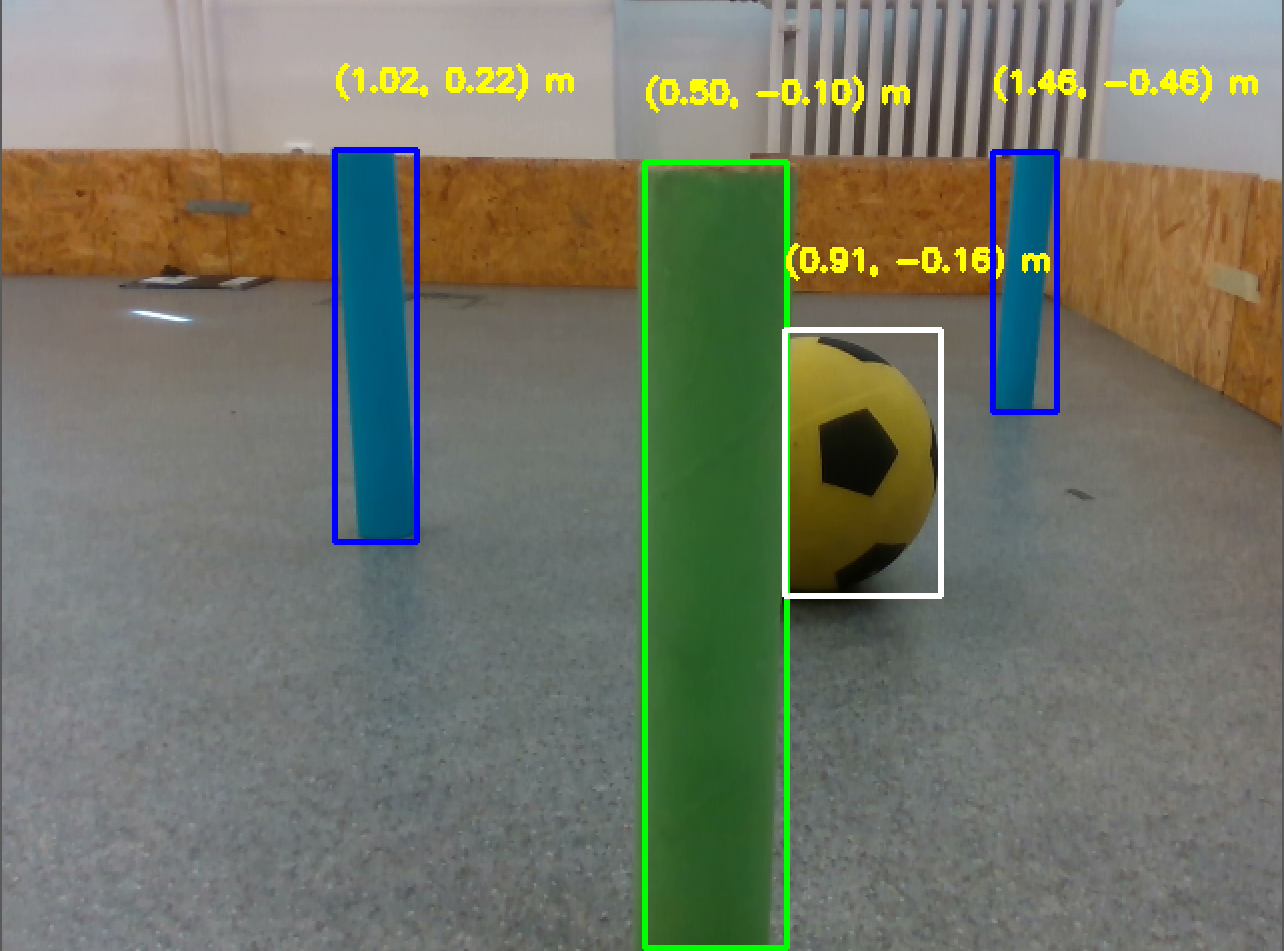
\includegraphics[width=0.5\textwidth]{pictures/detect.png}
    \caption{Obrázek z RGB kamery s rozpoznanými objekty}
    \label{fig:detect}
\end{figure}
\begin{figure}[H]
    \centering
    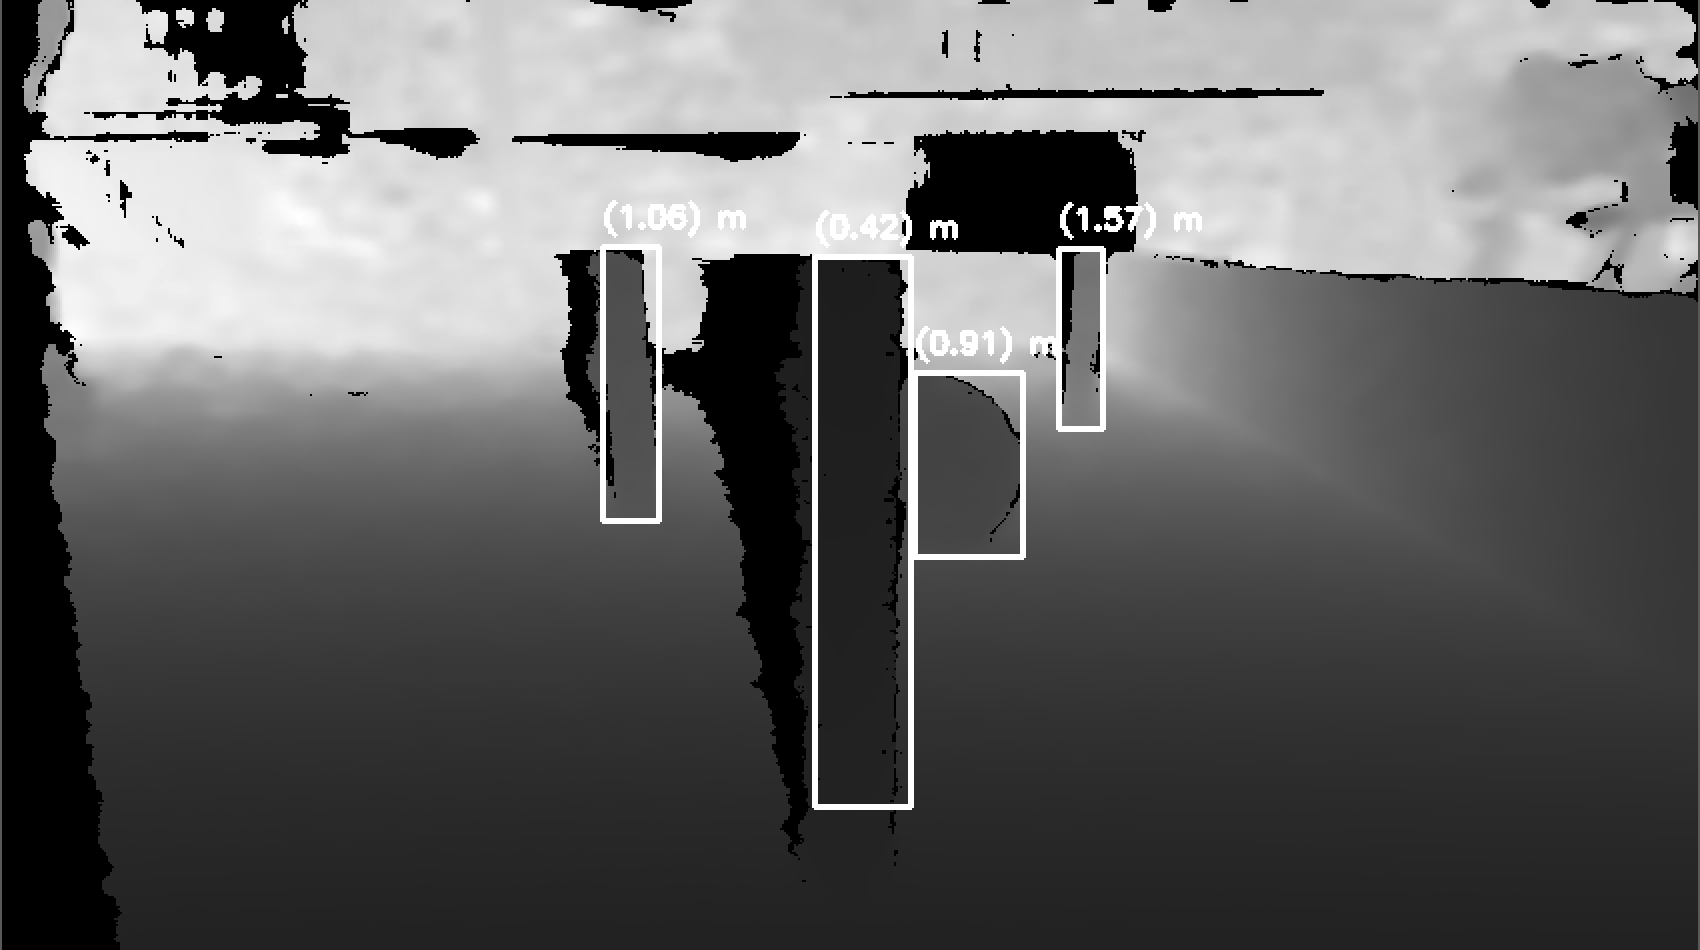
\includegraphics[width=0.7\textwidth]{pictures/depth_detect.png}
    \caption{Obrázek z hloubkové kamery s rozpoznanými objekty}
    \label{fig:depth_detect}
\end{figure}
Hloubková kamera vrací pouze pixeli s hloubkou. Aby byla poloha objektů spočítána co nejrychleji, pracujeme pouze s pixeli z hloubkové kamery (Obrázek \eqref{fig:depth_detect}), které jsou detekovány jako objekty z RGB kamery (Obrázek \eqref{fig:detect}).
Nejdříve vytvoříme transformační matici, která převadí mezi souřadnicemi kamery a hloubkové kamery. Poté se vypočítá median vzdáleností v bounding boxu, což řeší problém s obdelníky přesně nepasujícími na detekované objekty. 
Medián vzdálenosti přenásobíme konstantou 1.04, abychom korigovali nepřesnost depth kamery.
Pomocí K matice převedeme souřadnice z pixelů na reálné souřadnice vůči robotovi. Za souřadnice detekce se také přidá třída objektu.



\subsection{Lokalizace a mapování}
Jelikož je plocha, po které se pohybujeme rovná, je možné používat pouze 2D souřadnice. Pro lokalizaci robota a mapování používáme SLAM algoritmus z rodiny 
Kalman filtrů, kvůli nelinearitě transformace z globálních souřadnic do lokálních bylo potřeba použít Kalman filtr, který si umí s nelinearitami poradit. 
Tedy se nabízí dvě možnosti, Extended Kalman Filter (EKF) a Unscented Kalman Filter (UKF). Pro náš účel jsme zvolili UKF, který je přesnější a při malém počtu landmarků není výpočetně náročný.
\subsubsection{Unscented Kalman filter}
\label{sec:ukf}
Unscented Kalman Filter je založen na Unscented transformaci, která pomocí sigma bodů aproximuje nové normální rozdělení po transformaci. 
Sigma podle vzorce:
\begin{equation}
    \boldsymbol{\chi}_{i} = \begin{cases}
        \mathbf{\bar{x}} & i = 0 \\
        \mathbf{\bar{x}} + (\sqrt{(n + \lambda) \mathbf P})_{i-1} & 1 \leq i \leq n \\
        \mathbf{\bar{x}} - (\sqrt{(n + \lambda) \mathbf P})_{i-1} & n + 1 \leq i \leq 2n
    \end{cases}
\end{equation}
kde $\mathbf{\bar{x}}$ je odhad střední hodnoty, $\mathbf P$ je kovarianční matice a $\lambda$ je parametr, který určuje rozptyl sigma bodů a vypočítá se podle
\begin{equation}
    \lambda = \alpha^2(n + \kappa) - n
\end{equation}
kde $\alpha$ a $\kappa = 3 - n$ jsou vstupní parametry určující rozptyl sigma a $n$ je dimenze stavového vektoru kalman filtru. 
Pro výpočet Unscented transformace jsou poutřeba ještě váhy jednotlivých sigma bodů. 
Výpočet váhy aktuální střední hodnoty pro odhad nové je dělán podle: 
\begin{equation}
    w^{m}_0 = \frac{\lambda}{n + \lambda}
\end{equation}
Pro ostatní body pak podle 
\begin{equation}
    w^m_i = \frac{1}{2(n+\lambda)} \;\;\; i = 1...2n
    \label{eq:mean_weights}
\end{equation}
Výpočet váhy aktuální střední hodnoty pro odhad nové kovarianční matice je prováděn podle vzorce
\begin{equation}
   w^c_0 = \frac{\lambda}{n + \lambda} + 1 - \alpha^2 + \beta
\end{equation}
váhy pro ostatní body pak stejně jako pro odhad střední hodnoty, tedy podle (\ref{eq:mean_weights})
\\
Po vytvoření sigma bodů a jejich vah, je možné pomocí Unscented transformace určit nový odhad střední hodnoty a kovarianční matice pro funkční hodnoty dané transformace $f$ pro všechny sigma body.
\begin{equation}
    \begin{aligned}
    \boldsymbol{\mathcal{Y}} &= f(\boldsymbol{\chi}) \\
    \mathbf{\bar{x}} &= \sum_{i=0}^{2n} w^m_i\boldsymbol{\mathcal{Y}}_i \\
    \mathbf{\bar{P}} &= \sum_{i=0}^{2n} w^c_i{(\boldsymbol{\mathcal{Y}}_i-\mu)(\boldsymbol{\mathcal{Y}}_i-\mu)^\mathsf{T}}
    \end{aligned}
    \label{eq:ukf_transform}
\end{equation}
\\
Kalman filtr má pak dva hlavní kroky, predikci a aktualizaci.\\

Predikce je provedena pomocí funkce $f$ a sigma bodů. Sigma body se transformují do nového prostoru pomocí funkce $f$ a odhadne se nová střední hodnota a kovarianční matice.
Pro UKF se pak používá Unscented transformace (\ref{eq:ukf_transform}) pro výpočet nové střední hodnoty a kovarianční matice, 
navíc je k nové kovarianční matici přičtena matice $\mathbf Q$, která je matice šumu procesu. Dostaneme tedy
\begin{equation}
    \begin{aligned}
        \boldsymbol{\mathcal Y} &= f(\boldsymbol\chi) \\
        \mathbf{\bar x} &= \sum w^m\boldsymbol{\mathcal Y}  \\
        \mathbf{\bar P} &= \sum w^c({\boldsymbol{\mathcal Y} - \mathbf{\bar x})(\boldsymbol{\mathcal Y} - \mathbf{\bar x})^\mathsf T}+\mathbf Q \\
    \end{aligned}
    \label{eq:ukf_predict}
\end{equation}

Aktualizace je prováděna pomocí měření ze senzorů, je tedy potřeba převést sigma body do prostoru měření, 
to se provádí pomocí funkce $h$ a jelikož žádné měření není přesné, tak šum měření je modelován maticí $\mathbf R$.
Pro odhad nové střední hodnoty a kovarianční matice se používá 
\begin{equation}
    \begin{aligned}
        \boldsymbol{\mathcal Z} &=  h(\boldsymbol{\mathcal{Y}}) \\
        \boldsymbol\mu_z &= \sum w^m\boldsymbol{\mathcal{Z}} \\
        \mathbf y &= \mathbf z - \boldsymbol\mu_z \\
        \mathbf P_z &= \sum w^c{(\boldsymbol{\mathcal Z}-\boldsymbol\mu_z)(\boldsymbol{\mathcal{Z}}-\boldsymbol\mu_z)^\mathsf{T}} + \mathbf R \\ 
        \mathbf K &= \left[\sum w^c(\boldsymbol{\mathcal Y}-\bar{\mathbf x})(\boldsymbol{\mathcal{Z}}-\boldsymbol\mu_z)^\mathsf{T}\right] \mathbf P_z^{-1} \\
        \mathbf x &= \mathbf{\bar x} + \mathbf{Ky}\\
        \mathbf P &= \bar{\mathbf P} - \mathbf{KP_z}\mathbf{K}^\mathsf{T}
    \end{aligned}
\end{equation}

\subsubsection{SLAM struktura}
Stavový vektor ve SLAMu obsahuje pozici robota a pozice landmarků, které robot vidí, tedy 
\begin{equation}
    \mathbf x = \begin{bmatrix}
        x \\
        y \\
        \theta \\
        x_1 \\
        y_1 \\
        x_2 \\
        y_2 \\
        \vdots \\
        x_n \\
        y_n 
    \end{bmatrix}
\end{equation}
kde $(x,y, \theta)$ je pozice robota a $(x_i,y_i)$ je pozice $i$-tého landmarku.
Jelikož máme více typů landmarků, které se liší svojí třídou, je potřeba mít pro každý landmark uloženou třídu mimo stavový vektor, 
jelikož jejich chování na ní není závislé a zbytečně by se zvedala dimenze stavového vektoru.

\subsubsection{Predikce Kalman filtru ve SLAMu}
Predikce může být provedena podle fyzikálního modelu robota v závislosti na kontolních vstupech $\mathbf u$, to je však v našem případě zbytečné,
jelikož robot nabízí odometrii, která může model nahradit. Jelikož polohy landmarků se nemění v čase, mění se pouze poloha robota. Dostaneme tedy
\begin{equation}
    f(\mathbf x,\mathbf u) = \mathbf x + \begin{bmatrix}
                                    \Delta x \\
                                    \Delta y \\
                                    \Delta \theta \\
                                    0 \\
                                    0 \\
                                    \vdots \\
                                    0
                                \end{bmatrix}
\end{equation}
Abychom zíkali pouze rozdíly z odometrie bez restartování integrace v robotovi v každé iteraci, musíme si uchovávat poslední odometrické hodnoty, označení $n-1$, a počítat rozdíly mezi nimi.
V lokálních souřadnicích robota pak dostaneme 
\begin{equation}
    \begin{bmatrix}
        \Delta x_l \\
        \Delta y_l \\
        \Delta \theta_l \\
    \end{bmatrix} = 
    \begin{bmatrix}
        (x_{n} - x_{n-1})\cos(-\theta_{n}) + (y_{n} - y_{n-1})\sin(-\theta_{n}) \\
         -(x_{n} - x_{n-1})\sin(-\theta_{n}) + (y_{n} - y_{n-1})\cos(-\theta_{n})\\
        \theta_{n} - \theta_{n-1} \\
    \end{bmatrix}
\end{equation}
Poté je potřeba převést delty do globálních souřadnic, což je v tomoto případě další rotace
\begin{equation}
    \begin{bmatrix}
        \Delta x \\
        \Delta y \\
        \Delta \theta \\
    \end{bmatrix} = 
    \begin{bmatrix}
        \Delta x_l \cos(\theta) + \Delta y_l \sin(\theta) \\
         -\Delta x_l \sin(\theta) + \Delta y_l \cos(\theta)\\
         \Delta \theta_l \\
    \end{bmatrix}
\end{equation}
Nepřesnot odometrie je modelována maticí $\mathbf Q$, která má dimenzi stejnou jako stavový vektor, bude tedy z velké části nulová. Známe pouze odchylky pro jednotlivé proměnné, které jsou v našem případě $x$, $y$ a $\theta$, tedy

\begin{equation}
    \mathbf Q_c = \begin{bmatrix}
        \sigma_{x} & 0 & 0 & 0 & ... & 0\\
        0 & \sigma_{y} & 0 & 0 & ... & 0 \\
        0 & 0 & \sigma_{\theta} & 0 & ... & 0\\
        0 & 0 & 0 & 0 & ... & 0\\
        \vdots & \vdots & \vdots & \vdots & \ddots & \vdots \\
        0 & 0 & 0 & 0 & ... & 0\\
    \end{bmatrix}
\end{equation}
to však neodpovídá transformaci, která je prováděna, tedy je potřeba použít Jacobian pro transformaci
\begin{equation}
    \mathbf J = \begin{bmatrix}
        \frac{\partial x}{\partial x_l} & \frac{\partial x}{\partial y_l} & \frac{\partial x}{\partial \theta_l} & 0 & ... & 0\\
        \frac{\partial y}{\partial x_l} & \frac{\partial y}{\partial y_l} & \frac{\partial y}{\partial \theta_l} & 0 & ... & 0\\
        \frac{\partial \theta}{\partial x_l} & \frac{\partial \theta}{\partial y_l} & \frac{\partial \theta}{\partial \theta_l} & 0 & ... & 0\\
        0 & 0 & 0 & 0 & ... & 0\\
        \vdots & \vdots & \vdots & \vdots & \ddots & \vdots \\
        0 & 0 & 0 & 0 & ... & 0\\
    \end{bmatrix} = \begin{bmatrix}
        \cos(\theta) & \sin(\theta) & 0 & 0 & ... & 0\\
        -\sin(\theta) & \cos(\theta) & 0 & 0 & ... & 0\\
        0 & 0 & 1 & 0 & ... & 0\\
        0 & 0 & 0 & 0 & ... & 0\\
        \vdots & \vdots & \vdots & \vdots & \ddots & \vdots \\
        0 & 0 & 0 & 0 & ... & 0\\
    \end{bmatrix}
\end{equation}
Výsledná matice $ \mathbf Q$ pro predikci je tedy
\begin{equation}
    \mathbf Q = \mathbf J \cdot \mathbf Q_c \cdot \mathbf J^T
\end{equation}

\subsubsection{Aktualizace Kalman filtru ve SLAMu}
Pro krok aktualizace používáme detekce z kamery, které jsou statické, to znamená, že pouze sloupky. 
Ty jsou na vstupu do SLAMu v lokálních souřadnicích robota, a mají tvar $(x_l, y_l, třída)$, kde třída je barva sloupku.
Pro vytváření mapy a lokalizaci robota však poutřebujeme souřadnice v globálních souřadnicích, pro převod do globálních souřadnic použijeme
\begin{equation}
    \begin{bmatrix}
        x_g \\
        y_g \\
    \end{bmatrix} = 
    \begin{bmatrix}
        x_r + x_l \cos(\theta) - y_l \sin(\theta) \\
        y_r + x_l \sin(\theta) + y_l \cos(\theta) \\
    \end{bmatrix}
    \label{eq:local_to_global}
\end{equation}
kde $(x_r,y_r)$ je pozice robota, $(x_l,y_l)$ je pozice landmarku v lokálních souřadnicích a $\theta$ je úhel robota. \\
V Kalman filtru však musíme transformovat souřadnice landmarků z lokálních do globálních souřadnic, to se provádí pomocí 
\begin{equation}
    \begin{bmatrix}
        x_l \\
        y_l \\
    \end{bmatrix} =
    \begin{bmatrix}
        (x_g - x_r) \cos(\theta) + (y_g - y_r) \sin(\theta) \\
        - (x_g - x_r) \sin(\theta) + (y_g - y_r) \cos(\theta) \\
    \end{bmatrix}
    \label{eq:global_to_local}
\end{equation}

Nejdůležitějším krokem v aktualizaci z landmarků z kamery je správná asociace landmarků z kamery a landmarků v mapě. 
To provádíme pomocí eukleidovské vzdálenosti mezi landmarky z kamery a landmarky v mapě.
Pokud jsou splněny podmínky v (\ref{eq:association}) pro daný landmark z kamery $L^c_i$ a landmark z mapy $L^m_j$, pak je asociace provedena podle vzorce
\begin{equation}
    min_{j} \|L^c_{i} - L^m_{j} \| = min_{k} \|L^c_{k} - L^m_{argmin_{j} \|L^c_{i} - L^m_{j} \|}\| < \epsilon
    \label{eq:association} 
\end{equation}
kde $\epsilon$ je prahová hodnota pro vzdálenost mezi landmarky. 
Tím, že jsou třídy reprezentovány jako čísla, tak je možné použít k rozlišení tříd landmarků opět (\ref{eq:association}) a to tím způsobem, 
že třídy vynásobíme $10^6$ a tím přesuneme každou třídu do jiné roviny, avšak mezi landmarky stejné třídy budou vzdálenosti stejné.\\
Measurement fukce $h$ pro asociované landmarky je pouze převod landmarků z globálních do lokálních souřadnic podle (\ref{eq:global_to_local}).
\\
Measurement noise je modelováno maticí $\mathbf R$, která má stejnou dimenzi jako měření, tedy $2k$, kde $k$ je počet asociovaných landmarků.
Známe rozptyl pro jednotlivé landmarky v lokálních souřadnicích, tedy
\begin{equation}
    \mathbf R = \begin{bmatrix}
        \sigma_{x} & 0 & 0 & 0 & ... & 0\\
        0 & \sigma_{y} & 0 & 0 & ... & 0 \\
        0 & 0 & \sigma_{x} & 0 & ... & 0\\
        0 & 0 & 0 & \sigma_{y} & ... & 0\\
        \vdots & \vdots & \vdots & \vdots & \ddots & \vdots \\
        0 & 0 & 0 & 0 & ... & \sigma_{y}\\
    \end{bmatrix}
\end{equation}

\subsubsection{Aktualizace mapy}
\label{sec:update_map}
I když nám krok aktualizace Kalman filtru aktualizuje polohy jednotlivých namapovaných landmarků a polohu robota, je potřeba ještě přidat nové landmarky do mapy.
Jelikož nechceme kvůli stabilitě Kalman filtru mazat false detekce ze stavového vektoru a kovarianční matice, 
je potřeba rozlišit landmarky, které jsou opravdové a které jsou false detekce.\\
Z předchozího kroku máme asociované landmarky z kamery, pokud se nějaký landmark nepodařilo asociovat, tak je přidán do mapy uchazečů, 
která se nepoužívá na aktualizaci polohy ani kalman filtru, detekce jsou zde uchovány po maximální dobu $t_{max}$ od své poslední detekce. 
Pokud je zde landmark kratší dobu, je asociován s novýmy detekcemi v dalších iteracích a jehé je poloha aktualizována jako vážený průměr s váhou nové detekce $w_n = \frac{1}{1 + n}$, kde $n$ je počet detekcí daného landmarku.
Pokud je daný landnark viděn více než $n_{min}$ krát, je přidán do stavového vektoru a je rozšířena kovarianční matice s inicializací na 
\[
\mathbf P_{ln} = \begin{bmatrix}
    \sigma_{x} & 0 \\
    0 & \sigma_{y} \\
\end{bmatrix}
\]
je tedy ve tvaru 
\[
\mathbf P =
\begin{bmatrix}
    \mathbf P & \mathbf 0 \\
    \mathbf 0 & \mathbf P_{ln} \\
\end{bmatrix}
\]
a landmark je odstraněn z mapy uchazečů.
Jelikož se tím změní dimenze stavového vektoru je potřeba přepočítat parametry a vstupy Unscented transformace, tedy $\kappa$ a váhy jednotlivých sigma bodů podle postupu v kapitole \ref{sec:ukf}.\\


\subsection{Plánování}
Cílem plánovacího procesu v této úloze je generování trajektorií pro míč a následně pro pohyb samotného robota. Plánovací algoritmus využívá data získaná ze SLAMu, aktuální polohu míče a rovněž aktuální polohu a orientaci robota. Celý proces plánování lze rozdělit do čtyř hlavních oblastí, přičemž jednotlivé části a klíčové rozhodovací mechanismy jsou znázorněny na Obrázku \ref{fig:fig_plan_dig}. Výsledkem plánování je bod na trajektorii, který má robot navštívit jako první. V případě testovaní je plánovač také vrátit všechny vytvořené trajektorie. Tohoto režimu je využito v jednoduchém simulátoru. 

\begin{figure}
	\centering
	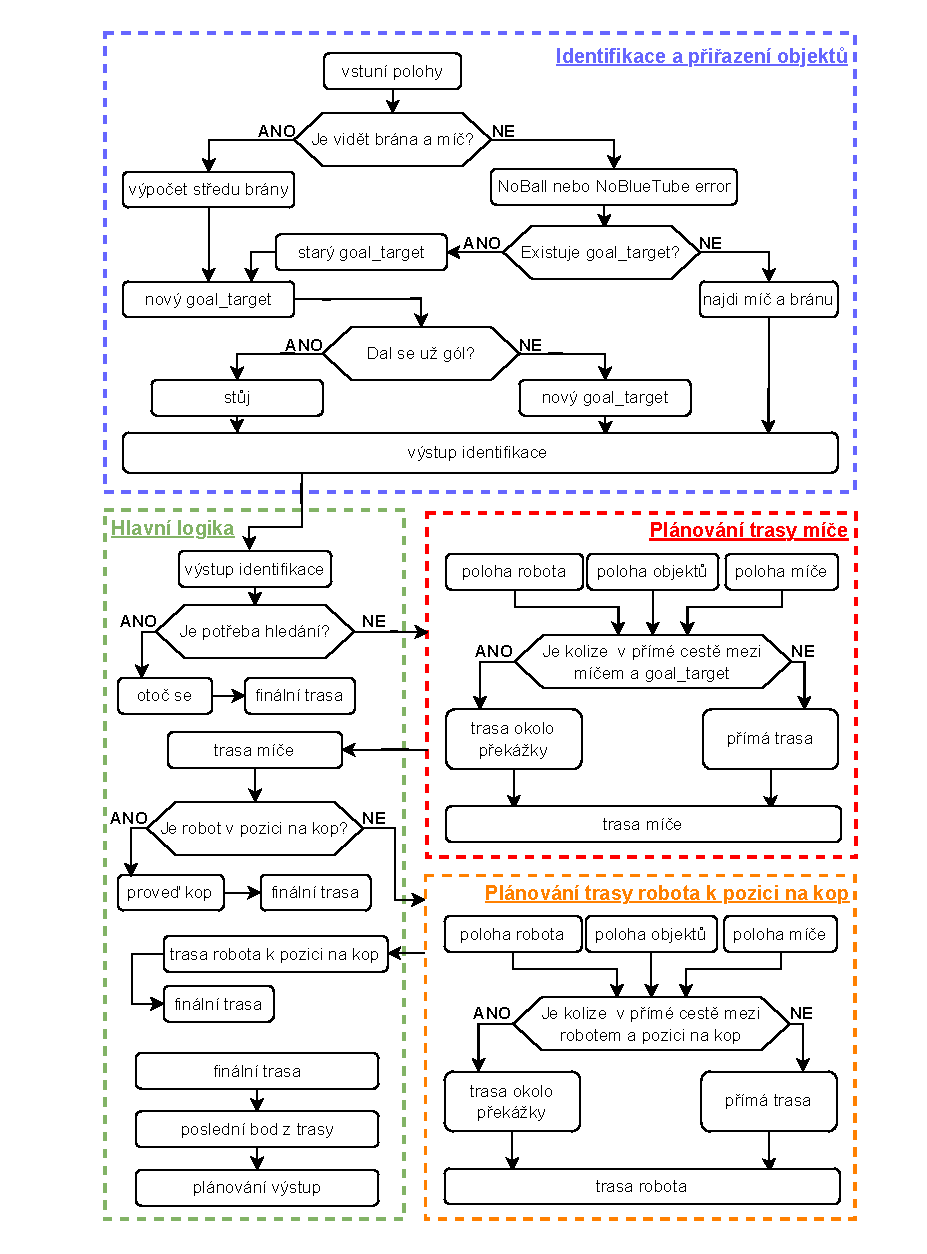
\includegraphics[width=\linewidth]{pictures/PlanningDiagram.pdf}
	\caption{Základní rozhodovací diagram plánovacího algoritmu}
	\label{fig:fig_plan_dig}
\end{figure}

\subsubsection{Identifikace a přeřazení objektů}
První fází plánovacího procesu je identifikace a přeřazení objektů, vyznačená modře na Obrázku \ref{fig:fig_plan_dig}. V této části dochází nejprve k načtení všech objektů vstupujících do plánovače a jejich roztřídění podle zadaných vlastností.\\
V případě, že jsou obě krajní kuželky brány detekovány, je následně vypočten její střed. Tento výpočet je proveden pomocí aritmetického průměru pozic krajních modrých tyčí branky. Výsledný bod je pak použit jako cílová pozice, do které se robot snaží dopravit míč. Pokud však brána není aktuálně viditelná a algoritmus nedisponuje informací o její pozici z předchozího běhu, fáze identifikace vrací pokyn k aktivnímu hledání brány.\\
V závěrečném kroku této fáze se ověřuje, zda již nedošlo ke vstřelení gólu. Detekce gólu je založena na porovnání vzdáleností míče od bodu ležícího před a za bránou. Tyto body jsou určeny pomocí projekce vektoru $\mathbf{w}$, který směřuje od robota ke středu branky, na vektor $\mathrm{v}$, reprezentující brankovou čáru. Tento výpočet je vyjádřen rovnicí \ref{eq:eq_proj}:
\begin{equation}
	proj_v(\mathbf{w})=\frac{\mathbf{w}\cdot\mathbf{v}}{\mathbf{v}\cdot\mathbf{v}}\cdot\mathbf{v}
	\label{eq:eq_proj}
\end{equation}
Na základě této projekce je následně spočten kolmo orientovaný vektor podle známého postupu, viz rovnice \ref{eq:eq_rej}:
\begin{equation}
	\mathbf{w_{per}}=\mathbf{w}-proj_v(\mathbf{w})
	\label{eq:eq_rej}
\end{equation}
Tento kolmý vektor je dále upraven (posunut a případně rotován) tak, aby směřoval jednak před branku, jednak za ni. Na základě těchto dvou bodů se následně rozhoduje, zda se míč nachází za brankovou čárou, a tedy zda došlo ke vstřelení gólu.\\

\subsubsection{Hlavní logika}
Druhou částí plánovacího procesu je hlavní logika, která je na Obrázku \ref{fig:fig_plan_dig} vyznačena zeleně. Tato část rozhodovacího mechanismu na základě informací z fáze identifikace a aktuální polohy robota určuje, kde se bude nacházet další cílový bod, na který má robot směřovat.\\

První možnou situací, která může nastat, je potřeba aktivního hledání brány a míče. V takovém případě je robot naváděn pomocí vektoru kolmého na svůj aktuální směrový vektor, což způsobí jeho rotaci na místě s cílem rozhlédnutí se.\\

Pokud jsou současně detekovatelné jak brána, tak i míč, přechází systém do fáze plánování trajektorie míče (blíže popsáno v následující části). Po úspěšném naplánování této trajektorie se ověřuje, zda se robot již nachází v pozici vhodné k provedení kopu. Tato situace nastává tehdy, pokud robot splňuje dvě podmínky:
\begin{itemize}
	\item 
	Robot se nachází v těsné, předem definované oblasti okolo bodu, ze kterého začíná akcelerace směrem k míči.
	\item
	Úhel mezi vektory spojujícími míč se středem brány a robota se středem brány je menší než stanovená prahová hodnota, čímž je zajištěna dostatečná zarovnanost směru kopu.
\end{itemize}
Pokud tyto podmínky nejsou splněny, je jako další cílový bod zvolen první bod z naplánované trajektorie, která má robota navést do pozice vhodné pro provedení kopu.\\
Pokud jsou splněny všechny požadované podmínky, je jako cílový bod pro pohyb robota zvolen koncový bod škálovaného jednotkového vektoru, který je umístěn do pozice míče a směřuje ke středu brány. Délka vektoru je zvolena tak, aby vyvolala prudší akceleraci robota, a tím došlo k provedení kopu. 

\subsubsection{Plánování trajektorie míče}
Třetí částí plánovacího procesu je plánování trajektorie míče, které je na Obrázku \ref{fig:fig_plan_dig} znázorněno červeně. Tato fáze pracuje s polohou všech objektů ve scéně – tj. se všemi barevnými trubkami, aktuální polohou míče a polohou robota.\\
Základní trajektorie je inicializována jako přímá spojnice mezi aktuální pozicí míče a středem brány. Následně je tato trasa ověřována z hlediska možných kolizí s překážkami, konkrétně se zelenými a červenými trubkami.\\
Detekce kolizí je založena na výpočtu vzdálenosti bodu od úsečky. Úsečka je definována vektorem $\mathbf{v}$, zatímco bod, jehož vzdálenost se vyhodnocuje, je reprezentován vektorem $\mathbf{w}$, který vznikne spojením příslušného bodu s počátečním bodem úsečky.\\
Nejprve je spočten parametr projekce bodu na přímku, která vznikne prodloužením dané úsečky, a to podle rovnice \ref{eq:eq_dis_line_proj}:
\begin{equation}
	t = \frac{\mathbf{w}\cdot\mathbf{v}}{\mathbf{v}\cdot\mathbf{v}}
	\label{eq:eq_dis_line_proj}
\end{equation}
Parametr $t$ určuje relativní pozici projekce bodu vůči délce úsečky. Pokud $t$ nabývá hodnot mimo interval $[0, 1]$, znamená to, že projekce bodu leží mimo úsečku, a vzdálenost se proto porovnává s bližším krajním bodem této úsečky.\\
Finální vzdálenost je následně spočtena pomocí Eukleidovské normy vektoru a porovnána s předem definovanou prahovou hodnotou, která slouží k detekci potenciální kolize.\\
V případě detekce kolize vrací funkce pro kontrolu kolizí také konkrétní problémový bod. Kolem tohoto bodu je následně vytyčeno kruhové okolí s volitelným poloměrem, do něhož nesmí plánovaná trajektorie míče zasahovat. Pro řešení této situace byla zvolena metoda obejití kruhové oblasti pomocí tečen. Tyto tečny definují novou trasu, která vede míč kolem překážky.\\

\begin{figure}
	\centering
	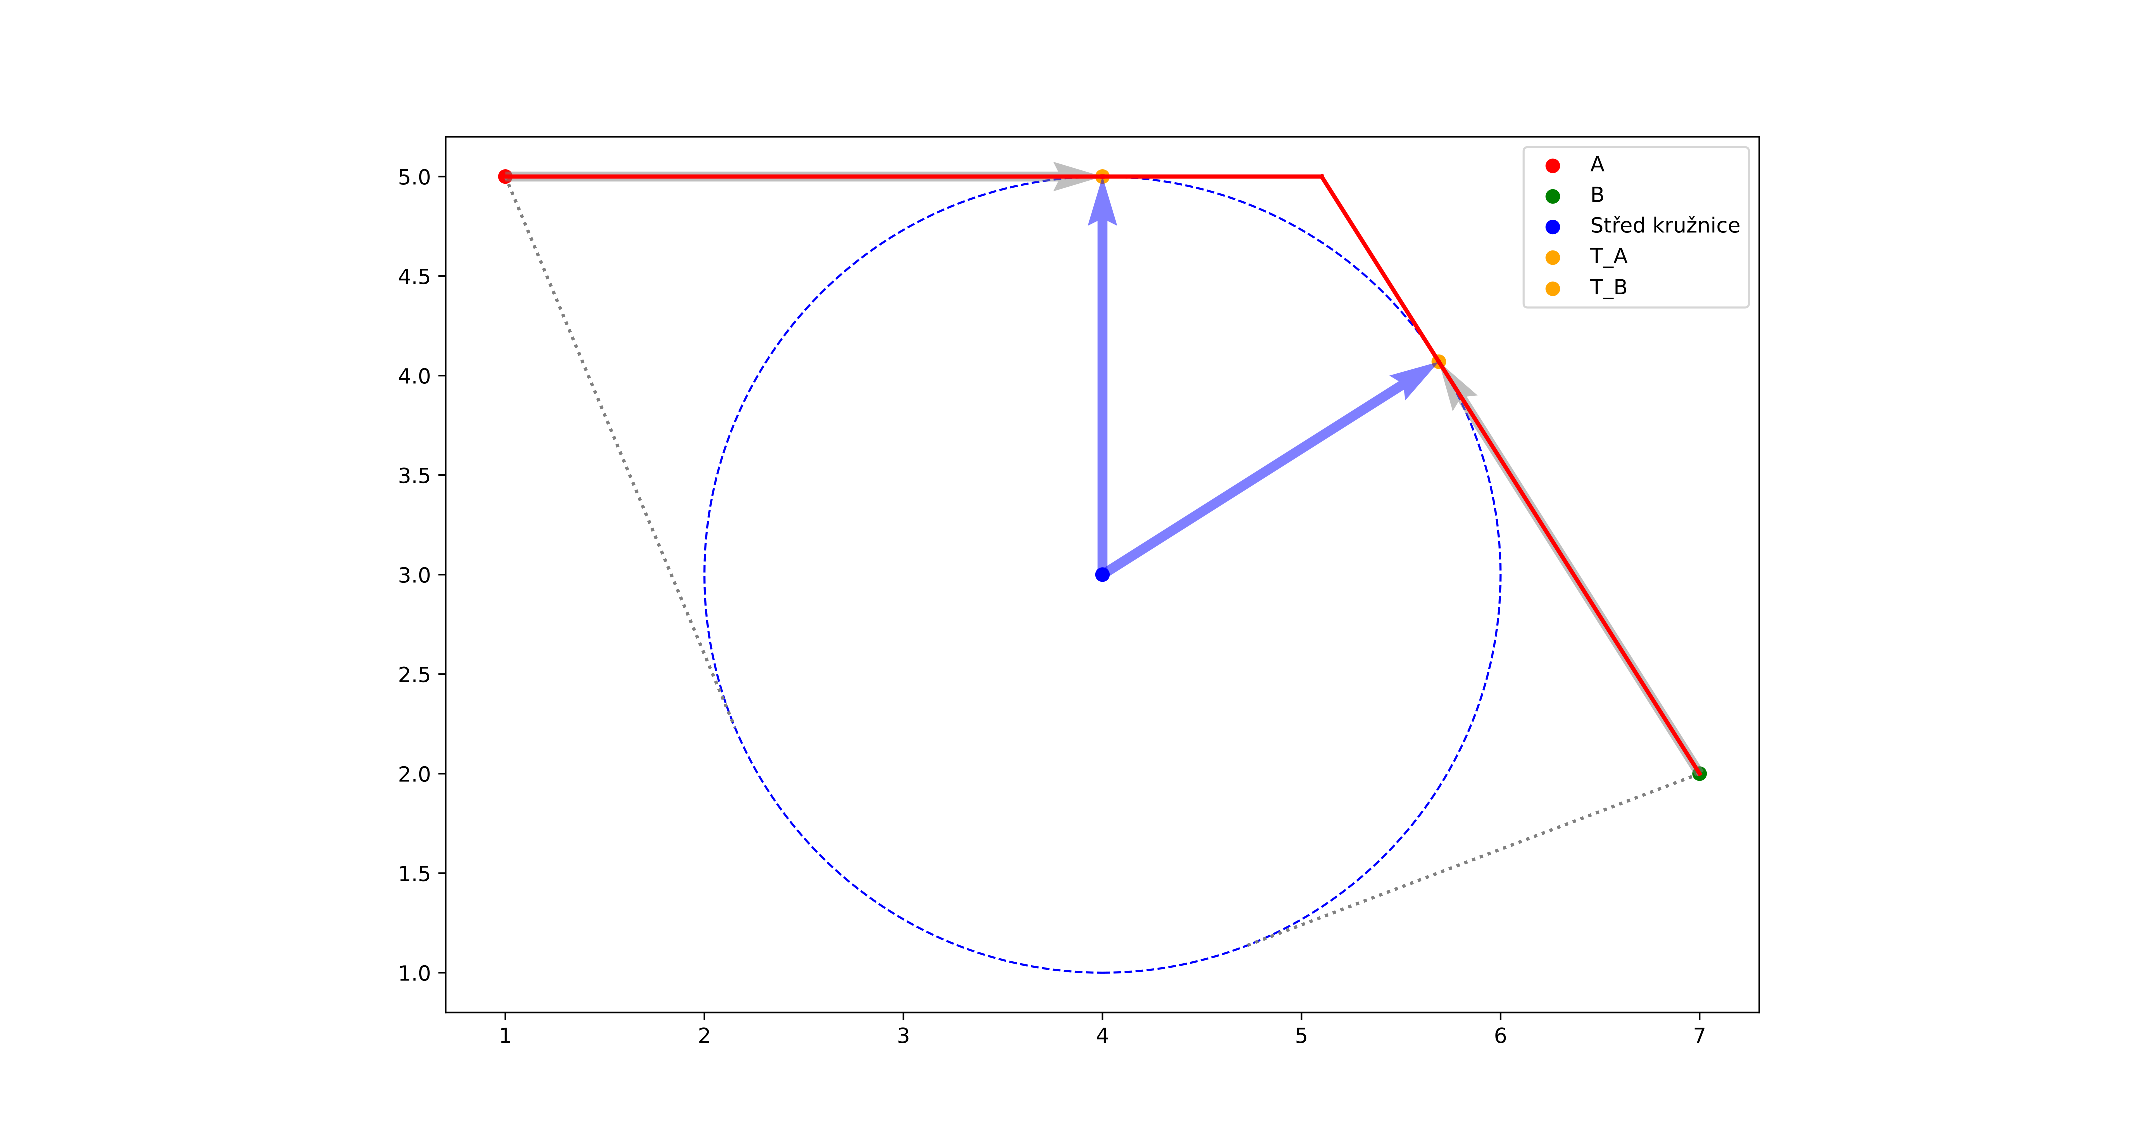
\includegraphics[width=\linewidth]{pictures/tangent_test-eps-converted-to.pdf}
	\caption{Znázornění trajektorie a pomocných vektorů metody obcházení pomocí tečen}
	\label{fig:fig_tangent}
\end{figure}

Funkce pro generování alternativní trajektorie akceptuje tři body: počáteční bod, koncový bod a střed kolizního okolí, spolu s poloměrem tohoto okolí. Nejprve jsou vygenerovány směrové vektory tečen ke kružnici, a to pro každý bod kromě středu, čímž vzniknou celkem čtyři tečny. Tyto tečny se vypočítávají pomocí rotace normalizovaného vektoru $d$, který spojuje daný bod se středem kružnice, o úhel $\alpha$. Tento úhel spolu svírá právě vektor $d$ a poloměr kružnice.\\
Úhel $\alpha$ je získán pomocí inverzní funkce kosinu, a to za předpokladu, že tečna je kolmá na poloměr, viz rovnice \ref{eq:eq_tan_angle}:

\begin{equation}
	\alpha = \arccos(\frac{r}{|d|})
	\label{eq:eq_tan_angle}
\end{equation} 

Pro každý bod existují dvě tečny, a proto je vektor $d$ rotován jak o úhel $+\alpha$, tak o úhel $-\alpha$. Výsledné jednotkové vektory tečen jsou dány rovnicemi \ref{eq:eq_tan_rot}:

\begin{equation}
	\begin{aligned}
		&\mathbf{d}_{\text{rot}} =
		\begin{bmatrix}
			\cos\alpha & -\sin\alpha \\
			\sin\alpha & \cos\alpha
		\end{bmatrix}
		\cdot \mathbf{d} \\
		&\mathbf{d}_{\text{-rot}} =
		\begin{bmatrix}
			\cos(-\alpha) & -\sin(-\alpha) \\
			\sin(-\alpha) & \cos(-\alpha)
		\end{bmatrix}
		\cdot \mathbf{d} \\
	\end{aligned}
	\label{eq:eq_tan_rot}
\end{equation}

Tyto jednotkové vektory jsou dále posunuty a škálovány tak, aby ukazovaly na konkrétní body na kružnici. Viz modré vektory na Obrázku \ref{fig:fig_tangent}.

Následně jsou vytvořeny čtyři možné kombinace vzniklých tečen a hledají se jejich průsečíky pomocí soustavy lineárních rovnic, viz rovnice \ref{eq:eq_inter}. Zde $\mathbf{v}_1$ a $\mathbf{v}_2$ představují směrové vektory obou tečen a $\mathbf{A}_1$, $\mathbf{B}_1$ jejich počáteční body:

\begin{equation}
	\begin{bmatrix}
		\mathbf{v}_1 & -\mathbf{v}_2
	\end{bmatrix}
	\begin{bmatrix}
		t \\
		s
	\end{bmatrix}
	=
	\mathbf{B}_1 - \mathbf{A}_1
	\label{eq:eq_inter}
\end{equation}

Polohu průsečíku $\mathbf{P}_{\text{inter}}$ lze poté spočítat dle rovnice \ref{eq:eq_line_inter}:

\begin{equation}
	\mathbf{P}_{\text{inter}} = \mathbf{A}_1 + t \cdot \mathbf{v}_1
	\label{eq:eq_line_inter}
\end{equation}

Pro výběr nejoptimálnější trajektorie je následně ze všech možností zvolena ta, která má nejmenší celkovou délku. Výsledná trajektorie je tvořena lomenou čarou procházející body počátku $\mathbf{A}_1$, průsečíkem tečen $\mathbf{P}_{\text{inter}_i}$ a koncovým bodem $\mathbf{B}_1$. Tato optimální trajektorie je v obrázku \ref{fig:fig_tangent} znázorněna červeně.

\subsubsection{Plánování trajektorie robota}

Poslední, čtvrtou částí plánovacího procesu je generování trajektorie pro pohyb robota. I v tomto případě je využita metoda vyhýbání překážkám pomocí tečen, jak byla popsána v předchozí kapitole. Zásadní rozdíl však spočívá v tom, že cílovým bodem zde není střed brány, ale tzv. shoot point – bod nacházející se za míčem na přímce spojující míč se středem brány.\\

Při plánování trajektorie k tomuto bodu je navíc do systému detekce kolizí zahrnuta i poloha míče, čímž se zamezí jeho nechtěnému kontaktu při přípravné fázi pohybu. Tato kontrola kolize s míčem je po dosažení cílového bodu deaktivována, aby bylo možné provést samotný kop.

\subsubsection{Simulátor}
Pro potřeby ladění plánovacího algoritmu byl implementován jednoduchý simulátor, který automaticky generuje náhodná rozložení trubek a polohu robota dle pravidel úlohy 3. Simulátor byl vytvořen v prostředí Pygame, které umožňuje snadnou vizualizaci a zároveň ovládání pomocí uživatelských vstupů z klávesnice. V aktuální verzi simulace je dostupný pouze manuální režim řízení, tedy ovládání robota pomocí klávesnice – konkrétně pomocí kláves W, S, A a D.\\
Pohyb míče je modelován pomocí zjednodušeného fyzikálního modelu zahrnujícího tření, jehož parametr byl laděn tak, aby simulované chování odpovídalo co nejvíce reálnému pohybu molitanového míče. Vzhledem k nelineárnímu a nepředvídatelnému chování reálného míče je však simulace míče vnímána spíše jen jako orientační.\\
Náhled simulátoru je zobrazen na obrázku \ref{fig:fig_sim_a}. Všechny objekty v simulaci jsou zobrazeny ve svých reálných rozměrech, přičemž hrací plocha o velikosti 5 × 5 metrů je přepočtena na velikost okna 1000 × 1000 pixelů. Robot je zobrazen červenou barvou, přičemž je u něj vykreslen směrový vektor a zorné pole (FOV – Field of View) pomocí černých čar. Červené vodorovné čáry vymezují oblast, ve které se nesmí nacházet žádné objekty s výjimkou modrých trubek.\\
Modrá čára znázorňuje plánovanou trajektorii pro střelbu, zatímco červená lomená čára reprezentuje trajektorii pohybu robota. Simulace běží na frekvenci 100 FPS (Frames per Second) a lze ji ukončit buď vstřelením gólu, nebo stiskem klávesy ESC.

\begin{figure}
	\centering
	\begin{subfigure}{0.45\linewidth}
			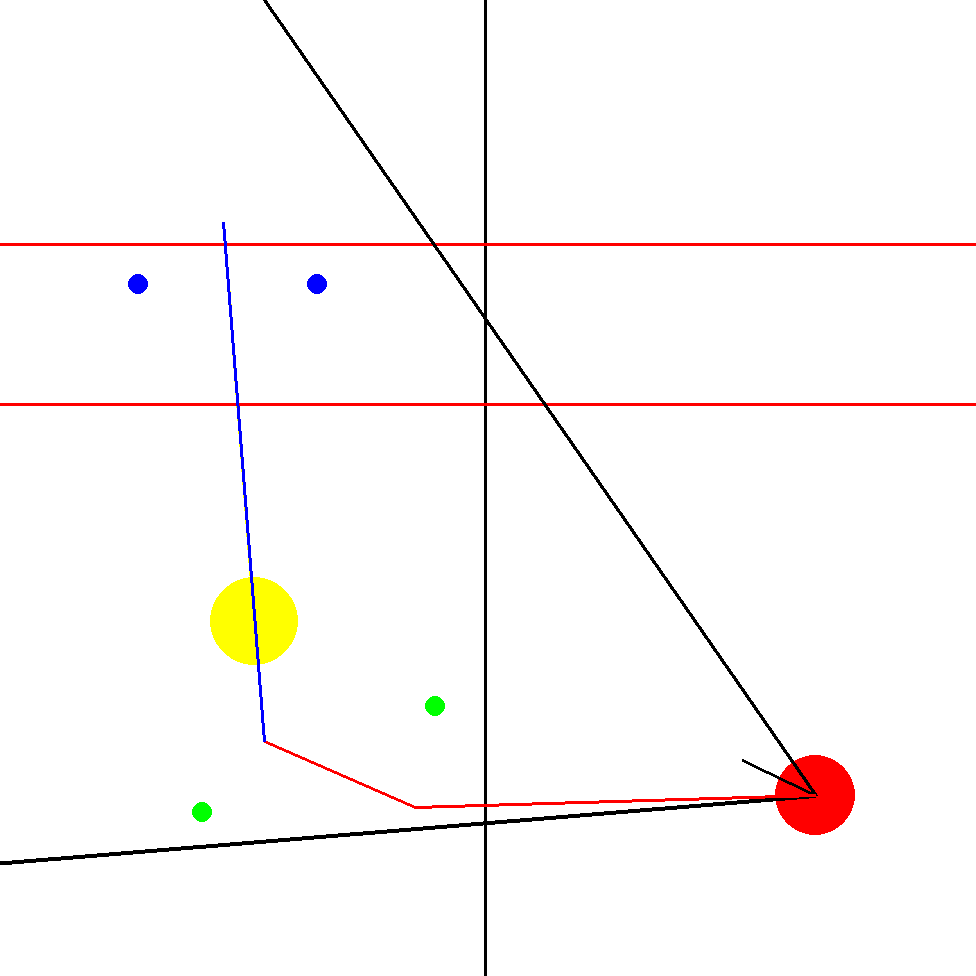
\includegraphics[width=\textwidth]{pictures/sim_002.png}
		\caption{Náhled jednoduchého simulátoru s nepřímou trajektorií}
		\label{fig:fig_sim_a}
	\end{subfigure}
	\begin{subfigure}{0.45\linewidth}
		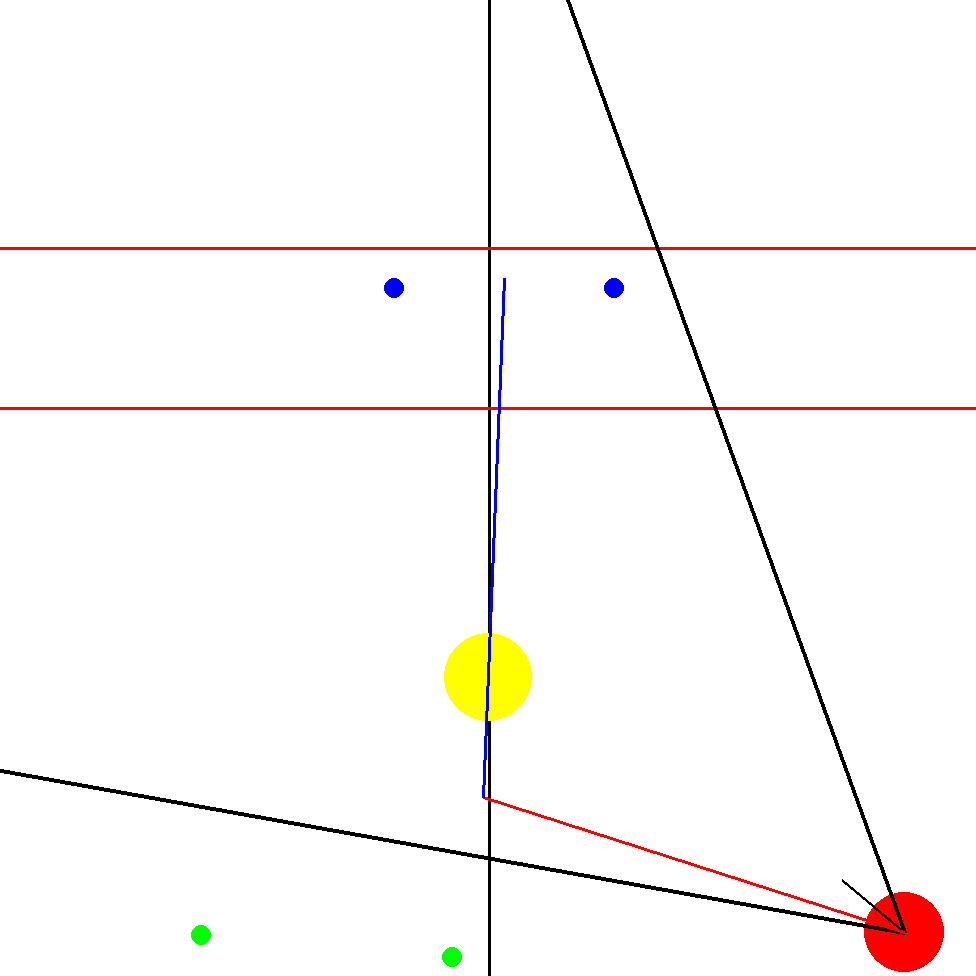
\includegraphics[width=\textwidth]{pictures/sim_001.png}
		\caption{Náhled jednoduchého simulátoru s přímou trajektorií}
		\label{fig:fig_sim_b}
	\end{subfigure}
	\caption{Náhled jednoduchého simulátoru pro úlohu 3}
\end{figure} 


\subsection{Pohyb}
Robotovi jde z path planningu cílová destinace, kam se má dostat v globálních souřadnicích v podobě $(x_g,y_g)$. To pomocí rovnice (\ref{eq:local_to_global}) převedeme do lokálních souřadnic $(x_l,y_l)$. 
Úhlovou rychlost robota počítáme pomocí vzorce 
\begin{equation}
    \omega = K_p * \arctan2(y_l,x_l)\\
    \label{eq:angular_velocity}
\end{equation}
Poté omezujeme rychlost na maximální povolenou rychlost robota $\omega_{max}$,
\begin{equation}
    \omega = \begin{cases}
        \omega_{max} & \omega > \omega_{max} \\
        -\omega_{max} & \omega < -\omega_{max} \\
        \omega & -\omega_{max} < \omega < \omega_{max}
    \end{cases}
\end{equation}
Lineární rychlost robota počítáme pomocí 
\begin{equation}
    v = \begin{cases}
        x_l (1 - (\frac{\omega}{\omega_{max}})^2) & x_l > 0 \\
        0 & x_l \leq 0
    \end{cases}
    \label{eq:linear_velocity}
\end{equation}
Poté rychlost omezíme maximální povolenou akcelerací robota $a_{max}$, tedy
\begin{equation}
    v = \begin{cases}
        v_{n-1} + \Delta t a_{max} & v \geq v_{n-1} + \Delta t a_{max} \\
        v_{n-1} - \Delta t a_{max} & v \leq v_{n-1} - \Delta t a_{max} \\
        v & v_{n-1} - \Delta t a_{max} < v < v_{n-1} + \Delta t a_{max}
    \end{cases}
\end{equation}
kde $\Delta t$ je časový krok mezi iteracemi a $v_{n-1}$ je rychlost robota v předchozí iteraci.\\
Potom už jen omezíme rychlost na maximální povolenou rychlost robota $v_{max}$, tedy
\begin{equation}
    v = \begin{cases}
        v_{max} & v > v_{max} \\
        -v_{max} & v < -v_{max} \\
        v & -v_{max} < v < v_{max}
    \end{cases}
\end{equation}

\section{Testování}
\subsection{Vidění}
Anotování obrázků obbélníky bez rotace představilo problém, který jde vidět v obrázku \eqref{fig:detected_image}. Díky zakřivení obrazu z kamery, obdelníky nesedí přímo na pilíře, což byl lehce vyřešitelný problém. Vzdálenost překážky bereme jako medián vzdáleností z obdelníku.
\begin{figure}[H]
    \centering
    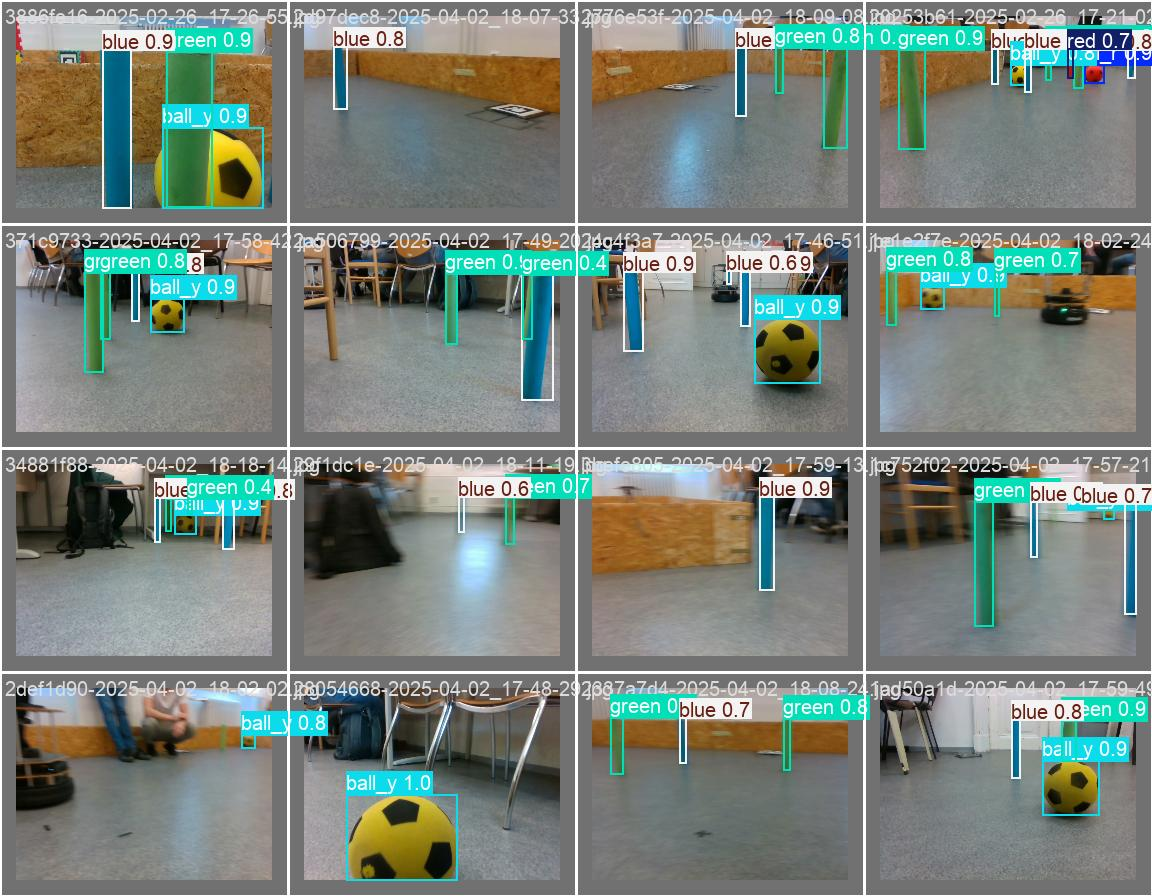
\includegraphics[width=0.7\textwidth]{pictures/rozpoznane.jpg}
    \caption{Rozpoznané objekty pomocí YOLO 11n při rozlišení 240p}
    \label{fig:detected_image}
\end{figure}

V obrázku \eqref{fig:detected_image} si ještě můžeme všimnout, že model dobře zvládá rozpoznávání objektů, které mají zaměnitelné barvy nebo tvar s objekty, které detekuje.
Model také například rozpoznal míč, když je z části za pilířem, nebo objekty, když jsou ve stínu pod stolem. Problémy občas tvoří objekty, které nebyly v trénovacím datasetu.
Boty s určitým vzorem mohou například být rozpoznány jako míč.

\subsection{SLAM}
Ve SLAMu bylo potřeba pro správné fungování nastavit parametry rozptyl v $\mathbf Q$ a $\mathbf R$ a také inicializační parametry pro Kalmanův filtr. 
Nejdříve jsme tedy z pozorování chování detekcí landmarků nastavili rozptyl pro jednotlivé landmarky na hodnotu $\sigma_x^2 = \sigma_v^2 = 0.2 \text{ m}^2$. Poté jsme spouštěli hlavní kontrolní smyčku, kde se SLAM aktualizoval pouze z detekcí, tedy bez kroku predikce.
Původně jsme měli nastavenou kovarianční matici na 
\[
\mathbf P = \begin{bmatrix}
    1 & 0 & 0 \\
    0 & 1 & 0 \\
    0 & 0 & 1 \\
\end{bmatrix}
\]
což vedlo k tomu, že se poloha byla ze začátku velmi chaotická. Po několika pokusech jsme došli k hodnotě 
\[
\mathbf P = \begin{bmatrix}
    0.1 & 0 & 0 \\
    0 & 0.1 & 0 \\
    0 & 0 & 0.1 \\
\end{bmatrix}
\]
Poté bylo potřeba odhadnout rozptyl pro odometrii, tedy $\mathbf Q$, abychom byli schopni spolehlivě odhadnout polohu robota, i když nevidíme žádné sloupky. Tam jsme se setkali s problémem, 
že byla použita moc velká nejistota pro úhel, takže poloha ve SLAMu nekorespodovala při otáčení s reálnou polohou robota. Po několika pokusech jsme došli k hodnotě $\sigma_\theta^2 = 0.001 \text{ rad}^2$ a pro polohu jsme došli k hodnotám $\sigma_{x}^2 = \sigma_{y}^2 = 0.2 \text{ m}^2$.\\

Ve SLAMu také původně nebyla žádné opatření proti false detekcím, což vedlo k tomu, že se SLAM snažil mapovat objekty, které nebyly v reálném světě, proto jsme přidali uchazeče od landmarky popsané v kapitole \ref{sec:update_map}. Po testování jsme došli k nastavení $t_{max} = 1$ a $n_{min} = 2$\\

Pro testování SLAMu jsme původně používali offline řešení pomocí matplotlib grafu na obrázku \ref{fig:slam_end}. \\

\begin{figure}[H]
    \centering
    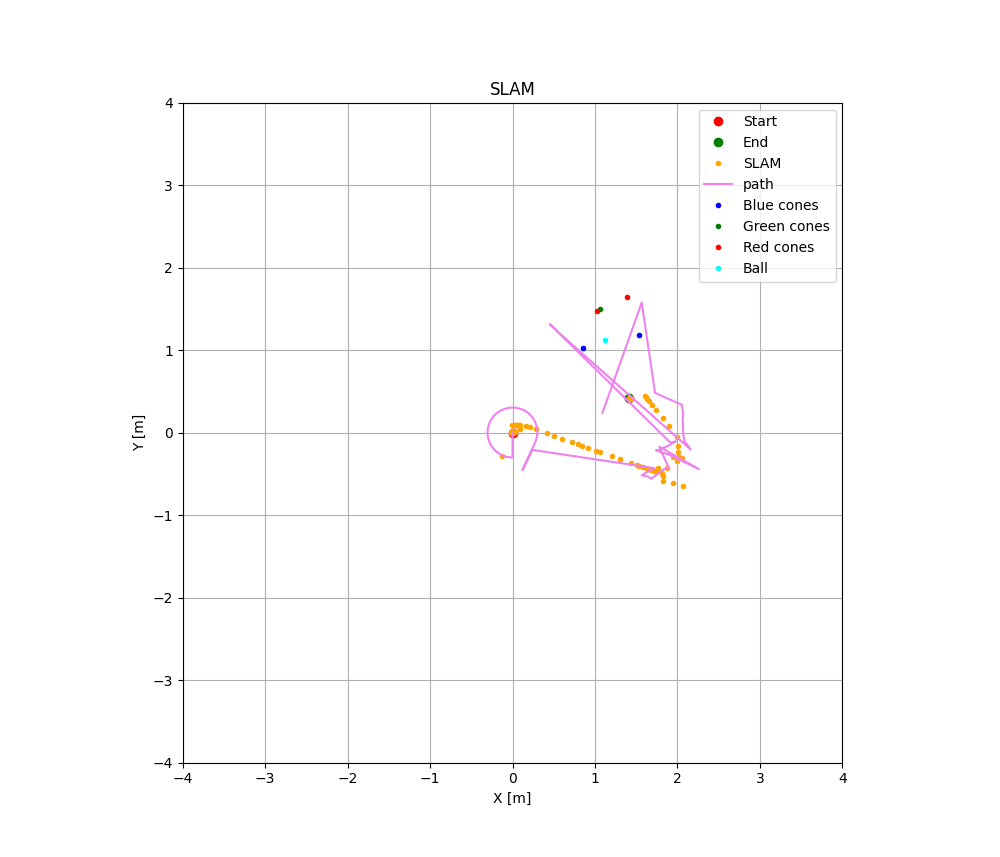
\includegraphics[width=0.7\textwidth]{pictures/slam3ok.png}
    \caption{Záznam proběhnuté trasy robota a detekovaných landmarků}
    \label{fig:slam_end}
\end{figure}

To však nebylo schopné dobře popsat chování v reálném čase, proto jsme použili vizualizaci v reálném čase pomocí opencv okna na obrázku \ref{fig:slam_in_game}.
\begin{figure}[H]
    \centering
    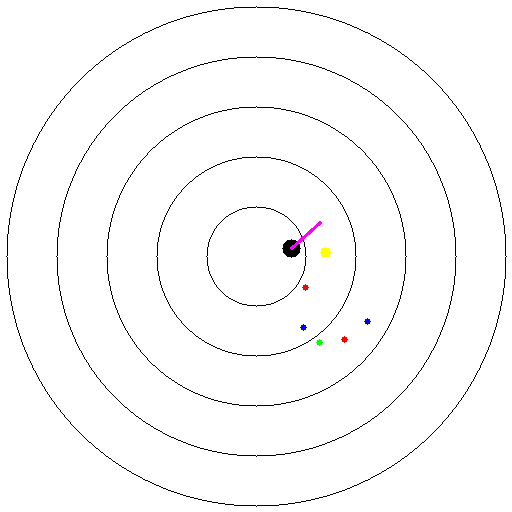
\includegraphics[width=0.5\textwidth]{pictures/map3.png}
    \caption{Vizualizace problému v průběhu řešení úlohy}
    \label{fig:slam_in_game}
\end{figure}

\subsection{Plánování}
Při testování plánovače byl zpočátku primárně využíván simulátor, ve kterém byla laděna logika programu. Při přechodu k testování na reálném robotu se však objevily časté problémy spojené s chováním míče. Vlivem jeho nepřesného tvaru a nerovností hracího povrchu dochází k výrazným odchylkám od naplánované trajektorie míče. Díky flexibilnímu chování plánovače je však možné tyto nepředvídatelné situace řešit přeplánováním trajektorie míče, čímž dochází ke korekci jeho pohybu. Pokud míč nedorazí do brány nebo se příliš odchýlí od požadované trajektorie, a zároveň nedojde ke kolizi s žádným z objektů, plánovač automaticky vygeneruje novou trajektorii. Tento proces se opakuje, dokud není dosaženo vstřelení gólu.\\
Toto chování bylo plně odladěno pro podmínky uvedené v zadání 2, kde se nevyskytují problémy spojené s kolizemi. Při testování na konfiguracích ze zadání 3 se však objevovaly potíže spojené s častou ztrátou viditelnosti objektů. To vedlo k častým změnám v plánované trajektorii, což mělo za následek prudké a dynamické pohyby robota. Tyto pohyby dále zvyšovaly nepřesnosti v měření a ztěžovaly stabilní navigaci. Možným řešením tohoto problému by bylo implementovat pokročilejší mechanismus pro dohledávání ztracených objektů.\\
Dalším problémem, který brání plynulé implementaci úlohy 3, je časté srážení míče s překážkovými trubkami při snaze je obstřelit. Tento problém je důsledkem již zmíněného chování míče. Možným řešením by bylo zavedení přesnějšího a přísnějšího polohování robota při střelbě. Tento přístup však naráží na komplikaci při určování přesných poloh, neboť při pouhém zmenšení tolerančních okolí pro jednotlivé navštívené body může docházet k zacyklení, kdy robot není schopen dosáhnout těchto bodů, kvůli časté malá změně jich polohy.\\
Plánovač není zcela dokonalý a v konfiguraci hracího pole ze zadání 3 se ukazuje jako velmi nespolehlivý v mnoha případech. Při použití konfigurace hracího pole ze zadání 2 však mnoho těchto problémů vymizí, což činí plánovač použitelným.
Dle testovaní byly nastaveny všechny důležité parametry plánovače tak, aby byl co nejvíce robustní a spolehlivý.\\
Prvním parametrem je poloměr okolí bodů pro detekci kolizí. Tento parametr $CLEARENCE$ byl nastaven na 0.5 m, což je dostatečně velká hodnota pro zajištění bezpečného objezdu překážek.\\
Druhým nastavovaným parametrem je $SHOOT\_STEPBACK$, což je vzdálenost, o kterou se robot posune zpět od míče před provedením kopu. Tento parametr byl nastaven na 0.8 m. Kvůli této větší vzálenosti je třeba zajistit, aby bylo za míčem dostatek prostoru pro provedení tohoto manévru.\\
Třetím parametrem je $SHOOT\_SCALING$, což je faktor, o který se zvětší délka směrového vektoru pro provedení kopu. Tento parametr byl nastaven na 2, což je dostatečně velká hodnota pro zajištění dostatečné akcelerace robota.\\
Čtvrtým parametrem je $HADING\_CHECK$, což je toleranční úhel pro provedení kopu. Tento parametr byl nastaven na 0.1746 rad, což je dostatečně hodnota pro zajištění dostatečné zarovnanosti směru kopu a zároveň zajišťuje stále dostatečnou vůli pro práci s nepřesnými daty.\\
Pátým a posledním důležitým parametrem, který byl lazen je $GOAL\_POX$, což je vzdálenost bodů od brankové čáry pro detekci gólu. Tento parametr byl nastaven na 0.1 m, což je dostatečně hodnota pro odrastranění šumu poloh a tudíž spolehlou detekci gólu.\\

\subsection{Pohyb}


\section{Závěr}

\begin{thebibliography}{5}

    \bibitem{YOLO}
    Ultralytics. \emph{YOLO Models}. Available at: \url{https://docs.ultralytics.com/models/}
    
    \bibitem{Ultralitics}
    Ultralytics. \emph{Ultralytics Documentation}. Available at: \url{https://docs.ultralytics.com/}
    
    \bibitem{ONNX}
    ONNX. \emph{Open Neural Network Exchange}. Available at: \url{https://onnx.ai/}
    
    \end{thebibliography}


\end{document}